%\VignetteIndexEntry{Prostar user manual}
%\VignetteKeywords{MassSpectrometry, Proteomics, DAPAR}
%\VignettePackage{Prostar}

\documentclass[12pt]{article}
\usepackage{soul}
\usepackage{url}
\usepackage[utf8]{inputenc}


\newcommand{\shellcmd}[1]{\\\indent\indent\texttt{\footnotesize\# #1}}
\newcommand{\bordurefigure}[1]{\fbox{\includegraphics{#1}}}

\RequirePackage[]{/Library/Frameworks/R.framework/Versions/3.4/Resources/library/BiocStyle/resources/tex/Bioconductor2}
\AtBeginDocument{\bibliographystyle{/Library/Frameworks/R.framework/Versions/3.4/Resources/library/BiocStyle/resources/tex/unsrturl}}
\usepackage[noae, nogin]{Sweave}

\bioctitle{\Biocpkg{DAPAR} and \Biocpkg{ProStaR} user manual}


\author{
Samuel Wieczorek\footnote{firstname.lastname@cea.fr} ,
Florence Combes$^\ast$,
Cosmin Lazar,
Quentin Giai Gianetto,\\
Laurent Gatto,
Alexia Dorffer,
Anne-Marie Hesse,
Yohann Coute,\\
Myriam Ferro,
Christophe Bruley
and Thomas Burger$^\ast$
}




\usepackage{Sweave}
\begin{document}

\Sconcordance{concordance:Prostar_UserManual.tex:Prostar_UserManual.Rnw:%
1 12 1 1 2 1 0 1 2 22 1 1 0 128 1 1 2 1 0 1 1 3 0 1 2 6 1 1 2 1 0 1 1 3 %
0 1 2 16 1 1 2 4 0 1 2 32 1 1 2 1 0 1 1 3 0 1 2 18 1 1 2 1 0 1 1 3 0 1 %
2 80 1 1 2 4 0 1 2 334 1 1 2 4 0 1 2 720 1 1 2 1 0 1 1 3 0 1 2 105 1 1 %
2 13 0 1 2 4 1}


\maketitle



%% Abstract and keywords %%%%%%%%%%%%%%%%%%%%%%%%%%%%%%%%
\vskip 0.3in minus 0.1in
\hrule
\begin{abstract}
\Biocpkg{DAPAR} (Differential Analysis of Protein Abundance with R) and 
\Biocpkg{ProStaR} (Proteomics and Statistics with R) are two Bioconductor 
packages that contain the necessary functions to analyze proteomics data 
(\Biocpkg{DAPAR}), as well as the corresponding graphical user interfaces 
(\Biocpkg{ProStaR}). This document guides the practitioner through the use of
\Biocpkg{DAPAR} (R command lines) and \Biocpkg{ProStaR} (click-button 
interface, so that no programming skill is required).
\end{abstract}
\vskip 0.1in minus 0.05in
\hrule
\vskip 0.2in minus 0.1in
%%%%%%%%%%%%%%%%%%%%%%%%%%%%%%%%%%%%%%%%%%%%%%%%%%%%%%%%%%

\newpage
\tableofcontents
\newpage

%%%%%%%%%%%%%%%%%%%%%%%%%%%%%%%%%%%%%%%%%%%%%%%%%%%%%%%%%%%%%%%%%%%%%%%%%%%%%%
\section{Introduction}\label{sec:intro}



\Biocpkg{DAPAR} and \Biocpkg{ProStaR} are a series of software dedicated to 
the processing of proteomics data. More precisely, they are devoted to the 
analysis of quantitative datasets produced in bottom-up discovery proteomics 
with a LC-MS/MS pipe-line (Liquid Chromatography and Tandey Mass 
spectrometry). The experiment package \Biocpkg{DAPARdata} is 
the companion package for \Biocpkg{ProStaR} and \Biocpkg{DAPAR}. It contains 
many datasets that can be used as example.\newline

\Biocpkg{DAPAR} (Differential Analysis of Protein Abundance with R) is an R 
package that contains all the necessary functions to:
\begin{itemize}
\item {Import/export a quantitative dataset.} Here, a quantitative dataset 
denotes a table where each protein is represented by a line and and each 
replicate is represented by a column; each cell of the table contains the 
abundance of a given protein in a given sample; the replicates are clustered 
into different conditions (or groups), and the purpose of the analysis is to 
isolate the few proteins the abundance of which significantly differ between 
the conditions (or groups).
\item {Compute and display meaningful statistics regarding the quantitative 
dataset.}
\item {Perform the various processing steps of a complete quantitative 
analysis}: (i) filtering and data cleaning; (ii) cross-replicate 
normalization; (iii) missing value imputation; {(iv) aggregation of peptide 
intensities into protein intensities;} (v) statistical tests and false 
discovery rate computation.
\end{itemize}

This package can be used on its own; or as a complement to the numerous 
Bioconductor packages (https://www.bioconductor.org/) it is compliant with; 
or through the \Biocpkg{ProStaR} interface.
\Biocpkg{ProStaR} (Proteomics and Statistics with R) is a web-interface based 
on Shiny (http://shiny.rstudio.com/) that provides Graphical User Interfaces 
(GUI) to all the \Biocpkg{DAPAR} functionalities, so as to guide any 
practitioner that is not comfortable with R programming through the complete 
quantitative analysis process.


In \Biocpkg{DAPAR}, a serie of functions may be called from two types of 
variables: a dataframe that contains quantitative data and an object of class 
MSnSet. The first case has been developped to make \Biocpkg{DAPAR} easier to 
use (in command line) for users who do not want to work with MSnSet files and 
to be compliant in the future with the Proline Suite 
(http://proline.profiproteomics.fr/).


%%%%%%%%%%%%%%%%%%%%%%%%%%%%%%%%%%%%%%%%%%%%%%%%%%%%%%%%%%%%%%%%%%%%%%%%%%%%%
%%%%%%%%%%%%%%%%%%%%%%%%%%%%%%%%%%%%%%%%%%%%%%%%%%%%%%%%%%%%%%%%%%%%%%%%%%%%%
%%%%%%%%%%%%%%%%%%%%%%%%%%%%%%%%%%%%%%%%%%%%%%%%%%%%%%%%%%%%%%%%%%%%%%%%%%%%%
\section{Installation}\label{sec:install}

%The installations of the two packages \Biocpkg{DAPAR} and \Biocpkg{ProStaR} 
%are made separately since \Biocpkg{DAPAR} can be run directly from a R 
%console. 
There are 3 ways to use \Biocpkg{DAPAR}:
\begin{itemize}
\item The first one is to use \Biocpkg{DAPAR} alone, through command lines or 
scripts. To do so, the user simply has to install \Biocpkg{DAPAR} on his/her 
own workstation, as instructed in Section~\ref{sec:daparalone};
\item The second one is to use \Biocpkg{DAPAR} along with its graphical 
interface \Biocpkg{ProStaR}, and to have them running on the user's station 
(referred to as stand-alone install). In such case, it is necessary to install
\Biocpkg{DAPAR} first, as instructed in Section~\ref{sec:daparalone}, and
\Biocpkg{ProStaR} then, as instructed in 
Section~\ref{sec:daparProstarstandalone};
\item In the case where several \Biocpkg{ProStaR} users who are not 
confortable with R (programming or installing), it is best to have a single 
version of \Biocpkg{DAPAR} and \Biocpkg{ProStaR} running on a shiny server 
installed on a Unix/Linux server. The users will use \Biocpkg{ProStaR} through 
a web browser, exactly if it were locally installed, yet, a single install has 
to be administrated. In that case, \Biocpkg{DAPAR} has to be classically 
installed (Section~\ref{sec:daparalone}), while on the other hand, the 
installation of \Biocpkg{ProStaR} is slightly different on a server 
(Section~\ref{sec:daparProstarserver}).
\end{itemize}
For a stand-alone use, both \Biocpkg{DAPAR} and \Biocpkg{ProStaR} can run on 
any operating system (Unix/Linux, Mac OS X and Windows) as long as R is 
installed. 
In any case (stand-alone or server), a recent version of R ($\geq$ 3.4) is 
needed.


\subsection{ProStaR (with DAPAR)}\label{sec:daparProstar}

\Biocpkg{ProStaR} can be run in two differents ways: standalone or server. The 
pre-requested packages described above have to be installed on the server if 
the user run a shiny-server to distribute \Biocpkg{ProStaR} or on a local 
machine if \Biocpkg{ProStaR} is run locally.



\subsubsection{Stand-alone version}\label{sec:daparProstarstandalone}

To run the stand-alone version, it is necessary to install the package in a 
directory where the user have read/write permissions. If the user have 
administrator privileges, then in a R console, enter:
\begin{Schunk}
\begin{Sinput}
> source("http://www.bioconductor.org/biocLite.R")
> biocLite("Prostar")
\end{Sinput}
\end{Schunk}

This step will automatically install the following packages: \CRANpkg{shiny}, 
\CRANpkg{reshape2}, \Githubpkg{jrowen/rhandsontable}, \CRANpkg{DAPARdata}, 
\CRANpkg{data.table}, \CRANpkg{DT}, \CRANpkg{shinyjs}, \CRANpkg{sm}, 
\CRANpkg{openxlsx}, \CRANpkg{shinyAce}, \CRANpkg{highcharter}.

Once the package is installed, to launch \Biocpkg{ProStaR}, then enter:
\begin{Schunk}
\begin{Sinput}
> library(Prostar)
> Prostar()
\end{Sinput}
\end{Schunk}

A new window of the default web browser opens. 


\subsubsection{Server version} \label{sec:daparProstarserver}
This version uses a Shiny Server 
(\url{https://github.com/rstudio/shiny-server}). It is a server program that 
makes Shiny applications available over the web. Please follow installation 
instructions if you do not have a server yet.

The first step is to install \Biocpkg{Prostar} as described in 
Section~\ref{sec:daparProstarstandalone} in order to have the dependencies 
installed.

Then, execute the following line in order to get the install directory of 
Prostar:

\begin{Schunk}
\begin{Sinput}
> installed.packages()["Prostar","LibPath"]
\end{Sinput}
\end{Schunk}


Change the owner of the shiny-server directory and log as shiny
\shellcmd{sudo chown shiny /srv/shiny-server}
\shellcmd{su shiny}\newline


Create a directory named \Biocpkg{ProStaR} in the Shiny Server directory with 
the user shiny as owner and then copy the Prostar files.\newline
\shellcmd{mkdir /srv/shiny-server/Prostar}
\shellcmd{chown -R shiny /srv/shiny-server/Prostar}
\shellcmd{cp -R prostarDir/ProstarApp/* /srv/shiny-server/ProStaR/.}

Then, complete the installation by copying the 'www' directory of 
\Biocpkg{ProStaR} and giving the following permissions:\newline
\shellcmd{cp -R inst/extdata/www /srv/shiny-server/Prostar/.}
\shellcmd{chmod 755 /srv/shiny-server/Prostar/www}\newline
\newline
Check if the configuration file of shiny-server is correct.\newline
For more details, please visit 
\url{http://rstudio.github.io/shiny-server/latest/}.

Now, the application should be available via a web browser at 
http://\emph{servername}:\emph{port}/Prostar.



\subsection{DAPAR (alone)}\label{sec:daparalone}


To install the package \Biocpkg{DAPAR} from the source file with administrator 
rights, start R and enter:

\begin{Schunk}
\begin{Sinput}
> source("http://www.bioconductor.org/biocLite.R")
> biocLite("DAPAR")
\end{Sinput}
\end{Schunk}

This step will automatically install the following packages:
\begin{itemize}
\item {From CRAN}: \CRANpkg{RColorBrewer}, \CRANpkg{Cairo}, \CRANpkg{png}, 
\CRANpkg{lattice}, \CRANpkg{reshape2}, \CRANpkg{tmvtnorm}, \CRANpkg{norm}, 
\CRANpkg{ggplot2}, \CRANpkg{imputeLCMD}, \CRANpkg{gplots}, \CRANpkg{openxlsx},
\CRANpkg{knitr}, \CRANpkg{cp4p}, \CRANpkg{doParallel}, \CRANpkg{scales},
\CRANpkg{stats}, \CRANpkg{grDevices}, \CRANpkg{vioplot}, \CRANpkg{sm}
\CRANpkg{graphics}, \CRANpkg{utils}, \CRANpkg{parallel}, \CRANpkg{openxlsx}, 
\CRANpkg{Matrix}, \CRANpkg{highcharter}
\item {From Bioconductor}: \Biocpkg{MSnbase}, \Biocpkg{preprocessCore}, 
\Biocpkg{impute}, \Biocpkg{limma}, \Biocpkg{pcaMethods}
\end{itemize}


\subsection{DAPARdata}\label{sec:DAPARdata}

The installation of the package \Biocpkg{DAPARdata} follows 
the classical way for Bioconductor packages. In a R console, enter:
\begin{Schunk}
\begin{Sinput}
> source("http://www.bioconductor.org/biocLite.R")
> biocLite("DAPARdata")
\end{Sinput}
\end{Schunk}

%%%%%%%%%%%%%%%%%%%%%%%%%%%%%%%%%%%%%%%%%%%%%%%%%%%%%%%%%%%%%%%%%%%%%%%%%%%%%%
%%%%%%%%%%%%%%%%%%%%%%%%%%%%%%%%%%%%%%%%%%%%%%%%%%%%%%%%%%%%%%%%%%%%%%%%%%%%%%
%%%%%%%%%%%%%%%%%%%%%%%%%%%%%%%%%%%%%%%%%%%%%%%%%%%%%%%%%%%%%%%%%%%%%%%%%%%%%%

\section{Navigating through the ProStaR interface}

\subsection{Overview of the interface}

\begin{figure}
\centering
\fbox{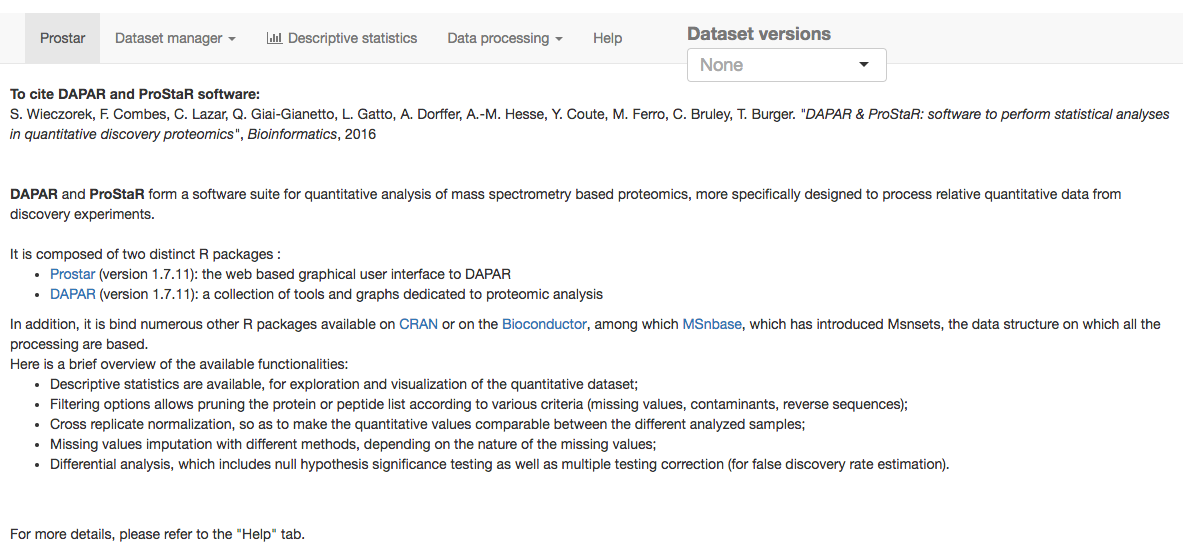
\includegraphics[width=0.65\textwidth]{images/defaultProstar1.png}}
\caption{Default screen of ProStaR}\label{fig:vuegal}
\end{figure}

{As illustrated on Fig.~\ref{fig:vuegal}, \Biocpkg{ProStaR} proposes a 
classical Graphical User Interface (GUI) to visualize and interact with the 
data. On the top, a navbar menu helps navigating through the various 
\Biocpkg{DAPAR} functionalities and running them. It is divided into five 
submenus:
\begin{itemize}
\item \textbf {ProStar}: The welcome page, depicted on Fig.~\ref{fig:vuegal}.
\item \textbf {Dataset manager}: It contains the tools to import and export 
datasets;
\item \textbf {Descriptive statistics}: It provides different visualization 
tools that are helpful to understand the dataset, and to picture the 
influence of the various processing;
\item \textbf {Data processing}: This is the heart of ProStaR, where all 
the \Biocpkg{DAPAR} functionalities can be accessed to; 
\item \textbf {Help}: A serie of informations about the software, 
associated references, etc.
\end{itemize}
}

{On the right hand side of the navbar menu, a dropdown menu referred to as 
"Dataset versions" makes it possible to navigate back through the history of 
the processing. Its use is detailed in Section~\ref{sec:availabledatasets}
}


%%%%%%%%%%%%%%%%%%%%%%%%%%%%%%%%%%%%%%%%%%%
%% Menu
%%%%%%%%%%%%%%%%%%%%%%%%%%%%%%%%%%%%%%%%%%%
\subsection{Dataset manager}
The "Dataset manager" allows the user to open, import or export quantitative 
datasets. \Biocpkg{ProStaR} and \Biocpkg{DAPAR} use the MSnSet format which 
is part of the package \Biocpkg{MSnbase}:
%~\cite{}.
It is either possible to load existing MSnSet files (see 
Section~\ref{sec:load}) or to import text (-tabulated) and Excel files (see 
Section~\ref{sec:import}). The "Demo mode" allows to load the datasets of the 
package \Biocpkg{DAPARdata} (see Section~\ref{sec:demomode}).


\subsubsection{Open MSnSet} \label{sec:load}
The user can upload a dataset that is already formated as an MSnSet file, by 
clicking on "Open MSnSet File" (see Fig.~\ref{fig:open}). This action opens a 
pop-up window, so as to let the user choose the appropriate file. Once the 
file is uploaded, a short summary of the dataset is shown, which includes the 
number of samples, the number of proteins in the dataset, the percentage of 
missing values and the number of lines which only contain missing 
values.\newline
\begin {figure}
\centering
\fbox{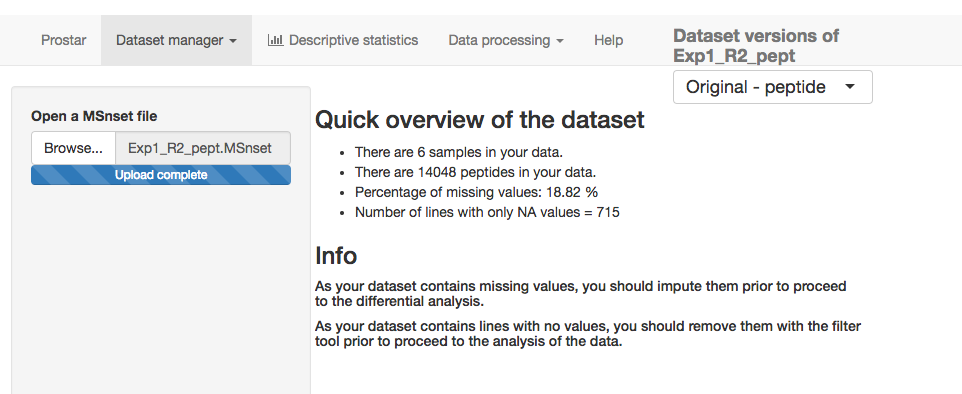
\includegraphics{images/open_msnset.png}}
\caption{Open a MSnSet file}\label{fig:open}
\end {figure}
{Once done, the menu of "Dataset versions" is updated to "Original - peptide" 
or "Original - protein" whether the file contains quantitative information 
about peptides or proteins (see Section~\ref{sec:availabledatasets}).} All 
the plots in the "Descriptive statistics" submenu (see 
Section~\ref{sec:descriptivestatistics}) become accessible and all the 
widgets to interact with \Biocpkg{ProStaR} are preloaded.

\hl{\bf Command line:} It is possible to open an MSnSet dataset directly in 
command line (\emph{i.e.} without \Biocpkg{ProStaR} interface), using 
function \Rfunction{readRDS()}.

{The user can find examples of MSnSet file in the 'extdata' directory 
of \Biocpkg{DAPARdata}. The user can find this directory by entering:\newline

\begin{Schunk}
\begin{Sinput}
> installed.packages()["DAPARdata","LibPath"]
\end{Sinput}
\end{Schunk}


% 
% Any user who wants to directly use \Biocpkg{DAPAR} in command line, 
%without \Biocpkg{ProStaR} interface, may upload an MSnSet file with 
%the \Rfunction{readRDS()} function:
% << runProstarStandalone>>=
% file <- "my_msnset_file"
% obj <- readRDS(file)
% @


\subsubsection{Import}\label{sec:import}
Alternatively, the user can create a quantitative dataset in the MSnSet 
format, on the basis of TSV (Tab Separated Values) or Excel files (in format 
xls or xlsx) that contain the results of a proteomics analysis. To do so, one 
has to click on "Convert data to MSnSet". Then, the right panel splits into 5 
tabs that guide the user through the procedure to create the MSnSet object. 
Let us describe the import format first, and the import procedure then. 

\noindent \textbf{Import data}\\
\noindent Data are imported through a text file (.txt) formatted as a column 
separated file, with tabulations (\textit{i.e.} "\textbackslash{}t" character) 
as column separator.
The first line of the text file contains the column names. A minimum of 4 
columns with quantitative values are necessary: As \Biocpkg{ProStaR} is made 
for label-free discovery proteomics, it is required to have \textit{a minima} 
2 conditions (or groups, or labels) to compare; moreover, 2 replicates per 
conditions are necessary, so that it is possible to compute a condition-wise 
variance. Regarding the quantitative values, the decimal separator is ".", 
and the intensities may be either log-transformed or not. It is also advised 
to have an additional columns that contains IDs (that is that gives a unique 
name to each line of the dataset). If such a unique ID does not appear in the 
dataset, one will be automatically generated.

Of course, it is possible to have more columns with quantitative values; as 
well as additional columns with other information. The latter ones will be 
considered as metadata when imported.

It is recommended to avoid special characters such as "$\sharp$", "@", "\$", 
"\%", etc. that are automatically removed. Similarly spaces in column names 
are replaced by ".".

If the dataset describes proteins, each line should correspond to one and 
only one protein. 
If the dataset describes peptides, each line should correspond to one and only 
one peptide. In addition, it is necessary to have a column that lists 
(separated by a ";") all the parent proteins of each peptide, as this piece of 
information is mandatory for the aggregation. It is also necessary that these 
parent proteins are describe by a unique ID (so as to avoid confusion between 
the proteins).

As an example, please find at the following address a dataset abstract that 
can be inspired from: \url{http://www.bioconductor.org/packages/release/bioc/
readmes/Prostar/README}. 


\noindent \textbf{Import procedure}\\
\noindent Several panels guide the user through the different steps of the 
procedure:

\textbf {Select file}: Select the CSV/txt or Excel (*.xls, *.xlsx) file to 
import (see Fig.~\ref{fig:imp1}). The file must contain a table where each line 
corresponds to a peptide or protein, except the first one which must contain 
the names of the colums. 
If the user chooses an Excel file, a dropdown menu appears and ask the user to 
select the spreadsheet containing the data. 

As it appears in Fig.~\ref{fig:imp1}, some options allows for 
specifying if data are related to peptides or proteins, if the abundance values
are already log-transformed or not \footnote{In \Biocpkg{DAPAR}, the analysis 
is always conducted on log-transformed data. They may have previously been 
transformed, but if not, then \Biocpkg{DAPAR} automatically performs the 
transformation. 
The user should not try applying any \Biocpkg{DAPAR} processing on data that 
are not log-transformed, for the result would be dubious.}, and also if $0$ 
and $NaN$ values should be replaced by \textbf{NA}. 
%These options are checked by default.
\begin {figure}
\centering
\fbox{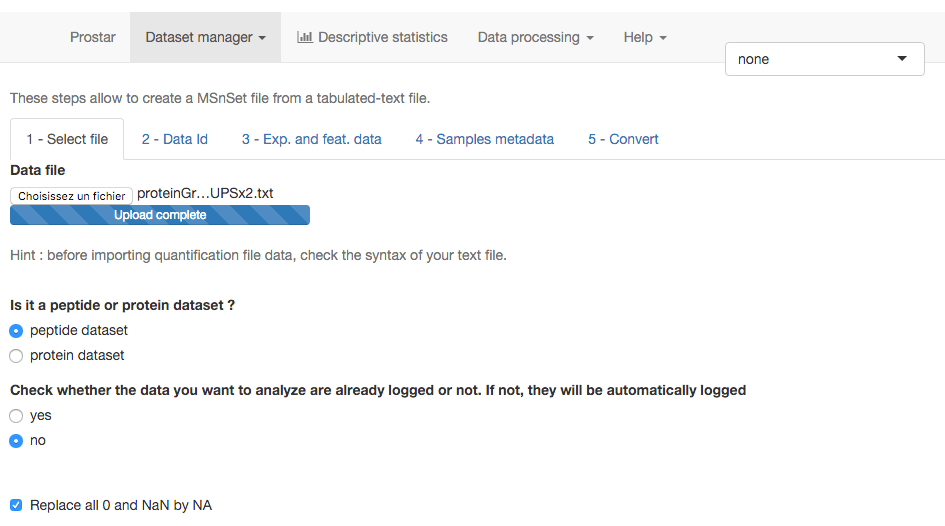
\includegraphics[width=\textwidth]{images/convert_selectfile.png}}
\caption{Importing an Excel file, tab 1.}\label{fig:imp1}
\end {figure}

{\textbf {Data ID}: This step is to set the column that corresponds to the 
unique ID of peptides or proteins. The user has two options: let 
\Biocpkg{ProStaR} creates such an ID by itself or choose among the columns 
available in the data file. If choosing the second option, then a drop-down 
menu appears and provides the list of the column names. A column corresponding 
to the unique ID of the peptides or proteins should be selected 
(see Fig.~\ref{fig:imp2}). If the column contains non unique IDs, a warning 
alerts the user and suggests him to choose another column.}
\begin {figure}
\centering
\fbox{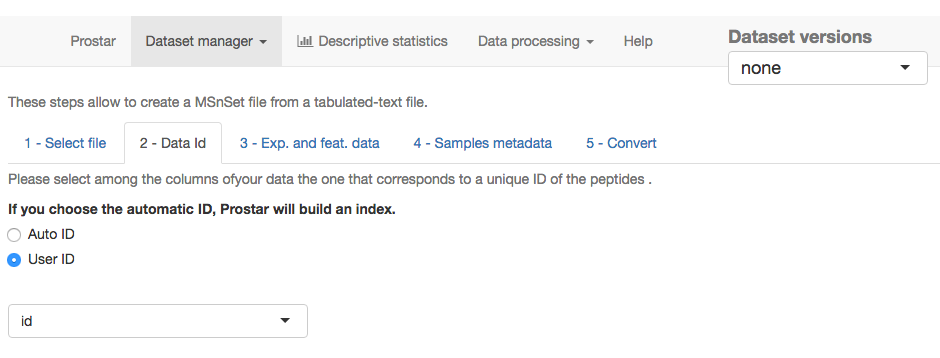
\includegraphics[width=0.75\textwidth]{images/convert_dataID.png}}
\caption{Importing a CSV file, tab 2.}\label{fig:imp2}
\end {figure}

\textbf {Exp. and Feat. data}: In the "Quantitative data" list, select (one 
after the other) the columns that correspond to the quantitative data. 
Each time the user selects an item in the list, it is moved up to the field 
above (see Fig.~\ref{fig:imp3}). If an item is selected by mistake, it can be 
removed by pressing on the SUPPR key.
\newline Please note that the decimal separator should be ".". 
\begin {figure}
\centering
\fbox{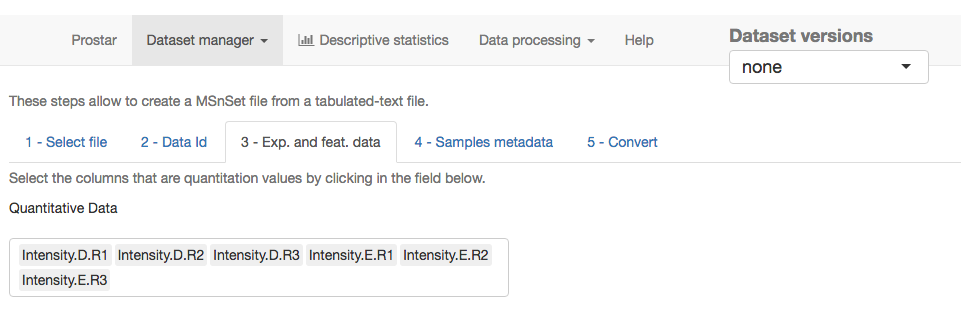
\includegraphics[width=\textwidth]{images/convert_exp_featdata.png}}
\caption{Importing a CSV file, tab 3.}\label{fig:imp3}
\end {figure}

\textbf {Sample metadata}: In this tab, the user fills the informations 
related to the samples, \textit{i.e.} the experimental design. The colum named 
\emph{Experiment} is filled by default with the name of the different samples. 
The user fills the other columns: 
\emph{Label} corresponds to the conditions of the experiment that will be 
compared during the differential analysis; \emph{Bio.Rep}, \emph{Tech.rep} 
and \emph{Analyt.Rep.} correspond respectively to the biological, technical 
and analytical replicates (Fig.~\ref{fig:imp4}). The column Label is 
mandatory (for the subsequent differential analysis), the other ones are 
optional.
\newline For the case of a peptide dataset, and in order to be able to agregate
the peptides intensities on proteins ones : there should be a column indicating,
for each peptide, the protein/s the peptide belongs to. If a peptide belongs to
more than one protein, proteins names should be separated by ";".  
\begin {figure}
\centering
\fbox{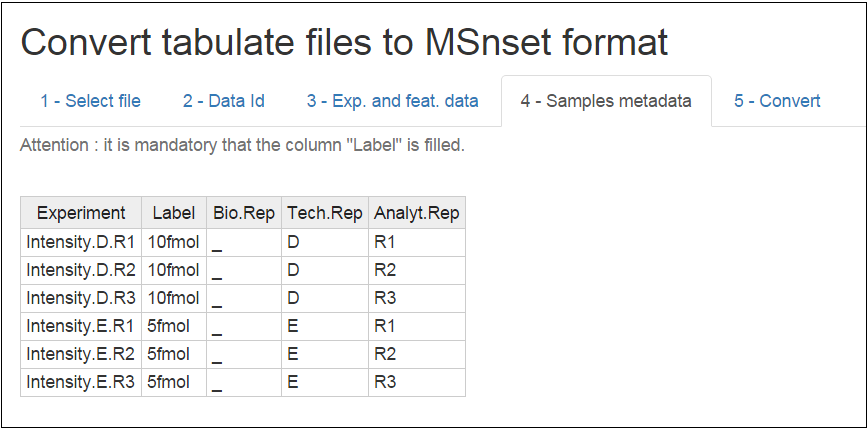
\includegraphics[width=0.67\textwidth]{images/convert_sampledata.png}}
\caption{Importing a CSV file, tab 4.}\label{fig:imp4}
\end {figure}

\textbf {Convert}: Finally, enter the name of the MSnSet to be created 
(Fig.~\ref{fig:imp5}) and click on "Convert data". The data are converted 
and automatically loaded in \Biocpkg{ProStaR}. The name of the file appears 
on the top of the left panel, above the menu.
\begin {figure}
\centering
\fbox{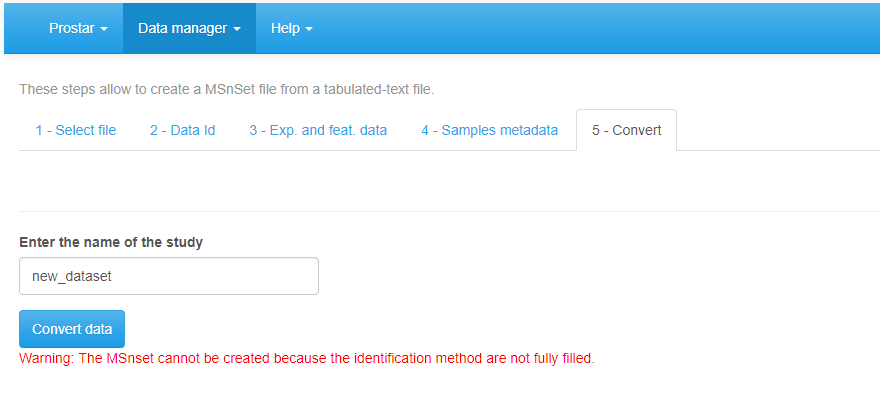
\includegraphics[width=0.9\textwidth]{images/convert_convert.png}}
\caption{Importing a CSV file, tab 5.}\label{fig:imp5}
\end {figure}


\hl{\bf Command line:} In \Biocpkg{DAPAR}, the function to create an MSnSet 
from a CSV file is \Rfunction{createMSnSet()}.


\subsubsection{Export}

\subsubsubsection{Export to a file}
Once an MSnSet has been created, it is possible to save it as a MSnSet binary 
object (so that next time, it is not necessary to create it, and a simple 
uploads makes it, as described in Section~\ref{sec:load}). It is also possible 
to export it as an Excel spreadsheet (in xlsx format). To do so, one simply 
goes on the corresponding tab and select the appropriate option 
(Fig.~\ref{fig:export}).


\begin {figure}
\centering
\fbox{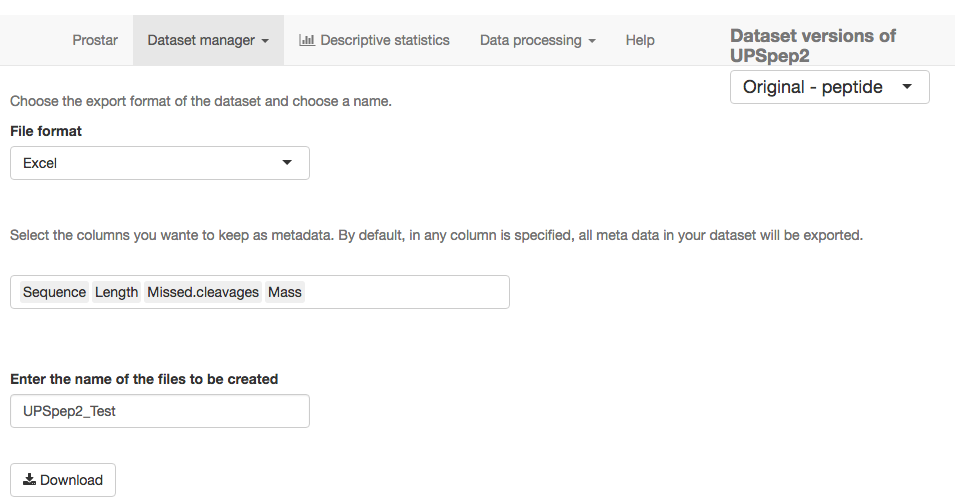
\includegraphics[width=0.9\textwidth]{images/export.png}}
\caption{Exporting to an Excel file.}\label{fig:export}
\end {figure}



%In case of Excel files, the user has to choose first the ID of the proteins. 
%The result is a file containing three sheets, one sheet per tab in the 
%MSnSet: expression data (quantitative data in our case), Feature Data and 
%Samples Data (see \Biocpkg{MSnbase} documentation~\cite{xxxxxx}).
%XXX The user chooses the format of the file and enter the name of the file. 
%Then, he clicks on the "Download" button XXX.

\hl{\bf Command line:} When working exclusively with \Biocpkg{DAPAR}, the 
functions are \Rfunction{writeMSnSetToExcel()} (to export in Excel format) 
and \Rfunction{saveRDS()} (to export in MSnSet format).


{The user can download the plots showed in \Biocpkg{Prostar} by 
right-clicking on the plot. A contextual menu appears and let the user 
choose either "Save image as" or "Copy image". In the latter case, he/she has 
to paste the image in appropriate software.}

\subsubsubsection{Export plots as report}



\subsubsection{Demo mode} \label{sec:demomode}

In order to facilitate first steps with Prostar, the "demo mode" menu allows 
the user to access the datasets contained in the package \Biocpkg{DAPARdata}. 
When the user chooses one of those datasets, it is automatically loaded in 
\Biocpkg{Prostar}. It can be used to easily test the various functionalities of
\Biocpkg{Prostar} (Fig.~\ref{fig:demomodeFig}).



\begin {figure}
\centering
\fbox{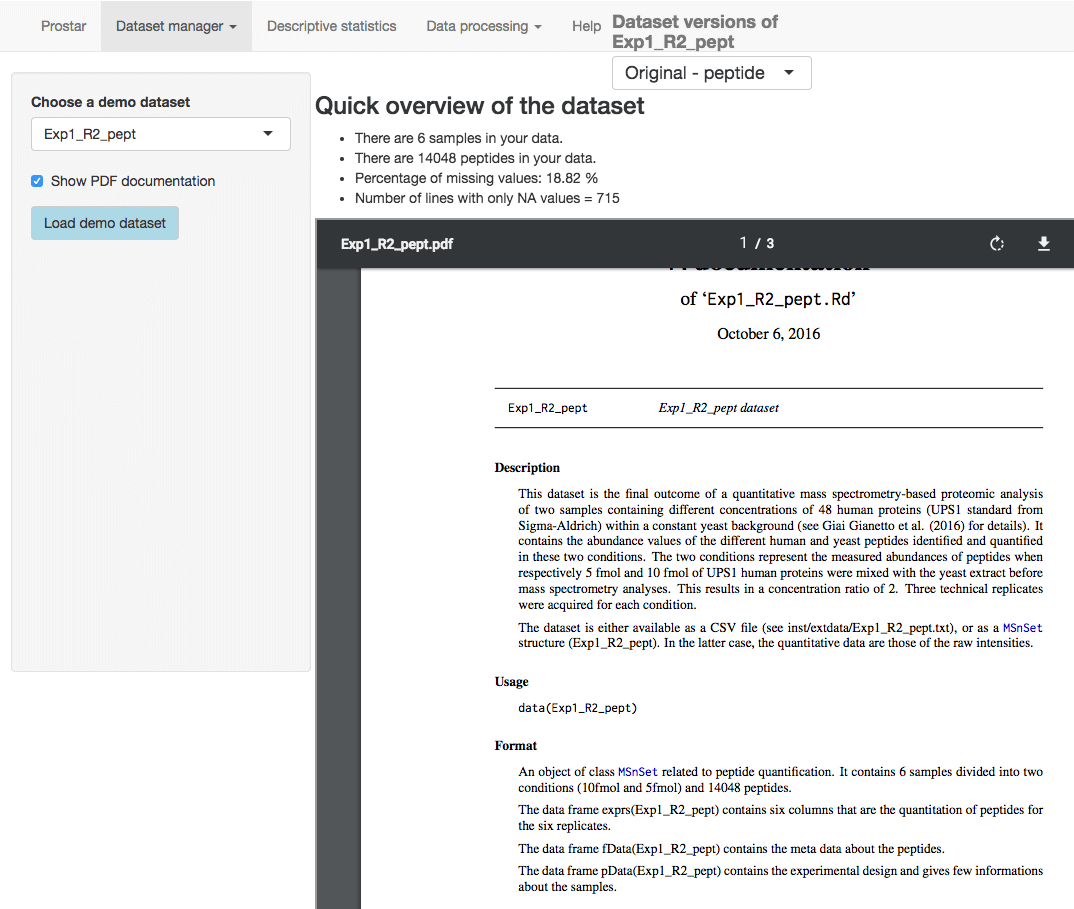
\includegraphics[width=0.9\textwidth]{images/demomode.png}}
\caption{Loadind a demo dataset.}\label{fig:demomodeFig}
\end {figure}


\subsubsection{Session log}\label{sec:sessionlog}

Each time the user validates a processing step (by clicking on the 
"Save <\emph{the\_step}>" button, see Section~\ref{sec:processingadataset}), 
the entire related information  (such as the method name and its parameters) 
is added to the table shown in the "Session log" tab 
(see Figure~\ref{fig:sessionlog}). Hence, this table is a history of how the 
data were processed during the session. 
Let us note that, if a dataset is processed, then saved and reloaded in a 
new session, the session log is naturally empty. To have a complete view on 
the previous processing applied to a given dataset, please refer to 
Section~\ref{sec:dataexplorer}).

\begin{figure}[b]
\centering
\fbox{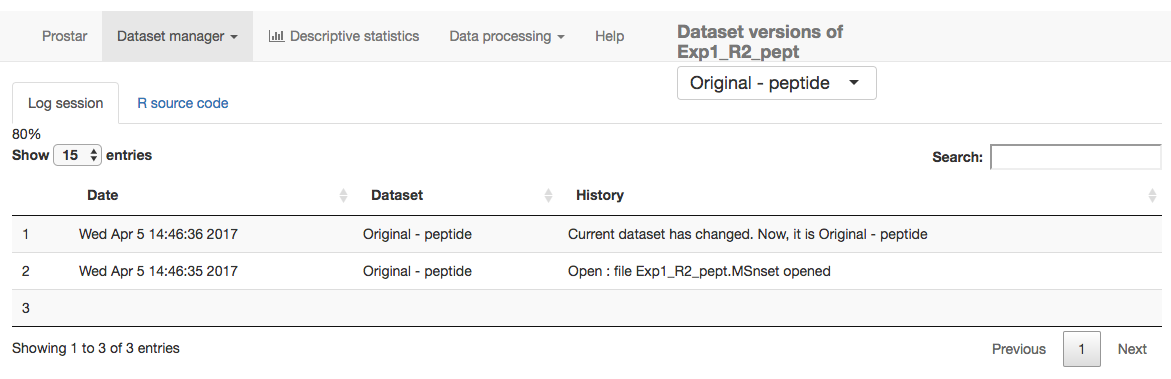
\includegraphics[width=0.75\textwidth]{images/logSession.png}}
\caption{Example of the log of a session in ProStaR.}\label{fig:sessionlog}
\end {figure}

Moreover, in the "R source code" tab, the user has access to the R commands 
(from DAPAR) that have been used to process its dataset 
(see Figure~\ref{fig:Rcode}). This code may be copy and paste in a R script to 
automate the analysis of a dataset.

\begin{figure}[b]
\centering
\fbox{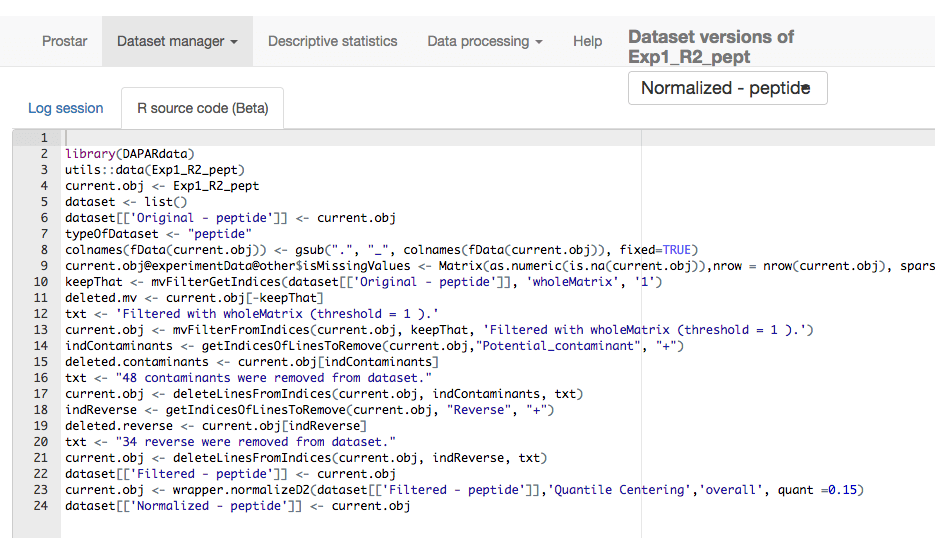
\includegraphics[width=0.75\textwidth]{images/Rcode.png}}
\caption{Example of the R code generated during a 
session in ProStaR.}\label{fig:Rcode}
\end {figure}


%%%%%%%%%%%%%%%%%%%%%%%%%%%%%%%%%%%%%%%%%%%
%% Menu
%%%%%%%%%%%%%%%%%%%%%%%%%%%%%%%%%%%%%%%%%%%
\subsection{Descriptive statistics}\label{sec:descriptivestatistics}

Several plots (one plot per tab) are proposed to help the user to have a 
quick and as complete as possible overview of his/her dataset. This menu is 
an essentiel element for the user to check that each processing step indeed 
gave the expected result.
%It is a crucial step to choose the statistical methods further.


\subsubsection{Missing value summary}


\begin {figure}
\centering
\fbox{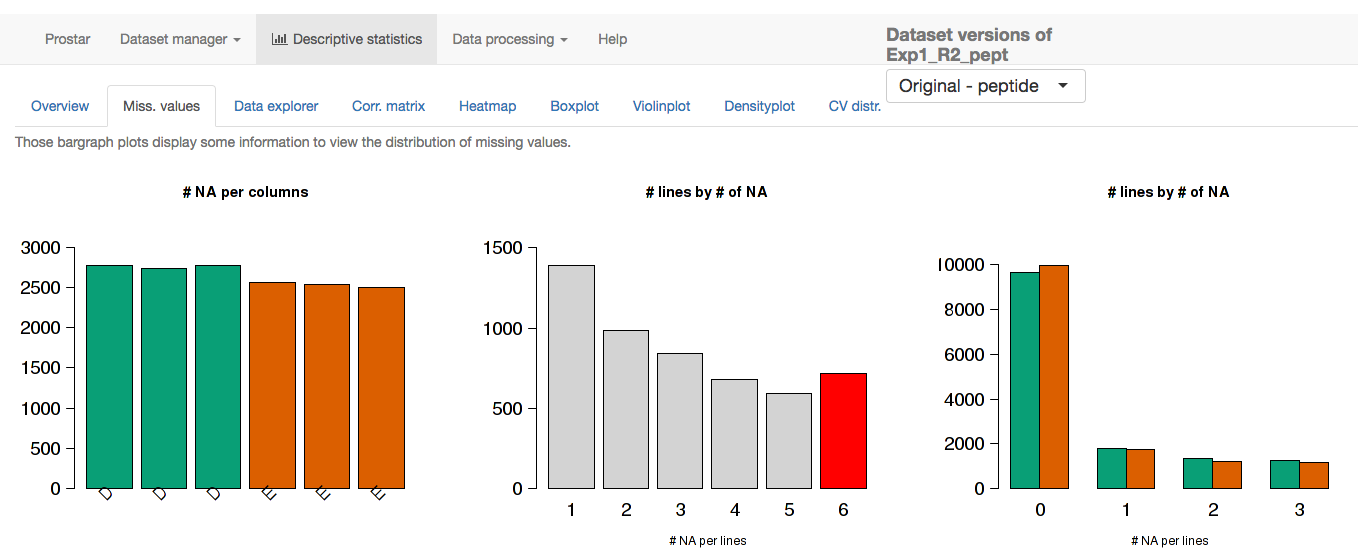
\includegraphics[width=0.75\textwidth]{images/desc_missValues.png}}
\caption{Histrograms for the overview of the missing values}\label{fig:sdmv}
\end {figure}

The barplot on the left represents the number of missing values in each 
sample. The different colors correspond to the different conditions (or label).
The histogram in the middle displays the distribution of missing values; the 
red bin counts the peptide or protein lines that only contains missing values 
(Fig.~\ref{fig:sdmv}).
{The barplot on the right shows the distribution of missing values per 
condition.}
%case where a line contains only missing values is colored in red. In this 
%example, there are 3 lines that contains 6 missing values.

\hl{\bf Command line:} In \Biocpkg{DAPAR}, the functions for these three 
plots are:
\begin{itemize}
\item for the dataframe parameter: \Rfunction{mvPerLinesHisto()}, 
\Rfunction{mvHisto()} and \Rfunction{mvPerLinesHistoPerCondition()},
\item for an object of class MSnSet: \Rfunction{wrapper.mvPerLinesHisto()}, 
\Rfunction{wrapper.mvHisto()} and 
\Rfunction{wrapper.mvPerLinesHistoPerCondition()}.
\end{itemize}
% end textcolor


\subsubsection {Data explorer}\label{sec:dataexplorer}
This panel allows viewing the content of the MSnSet structure. It is made of 
four tables, that are represented in a tab each. 
%by the three tables of the MSnSet format.
The first one, named "Quantitative data" contains quantitative values 
(see Fig.~\ref{fig:sdqv1}). The missing values are represented by empty cells.

\begin {figure}
\centering
\fbox{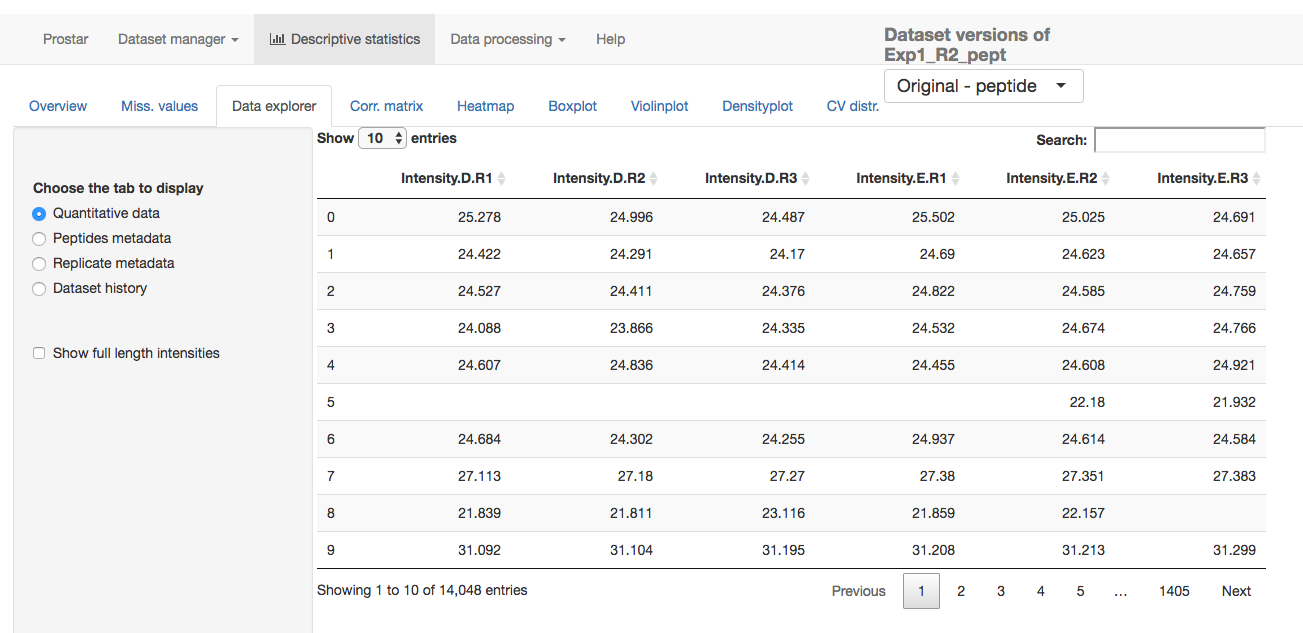
\includegraphics[width=0.80\textwidth]{images/desc_quantiData.png}}
\caption{View of quantitative data in the MSnSet dataset}\label{fig:sdqv1}
\end {figure}


The second tab is named "Analyte metadata". It contains the metadata of the 
proteins (see Fig.~\ref{fig:sdqv2}).

\begin {figure}
\centering
\fbox{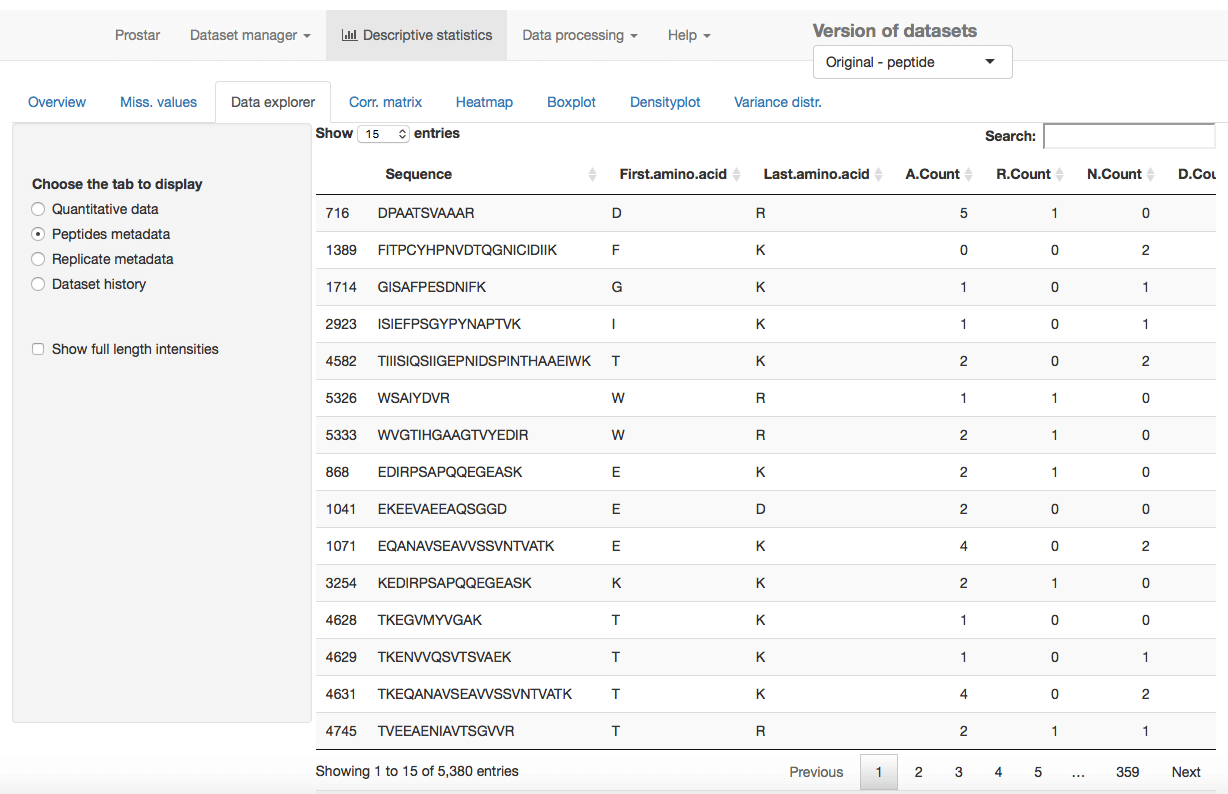
\includegraphics[width=0.80\textwidth]{images/desc_fdata.png}}
\caption{View of feature meta-data in the MSnSet dataset}\label{fig:sdqv2}
\end {figure}

The thrid tab is named "Replicate metadata". The information displayed here 
is the one entered by the user during the import step 
(see Fig.~\ref{fig:sdqv3}).

\begin {figure}
\centering
\fbox{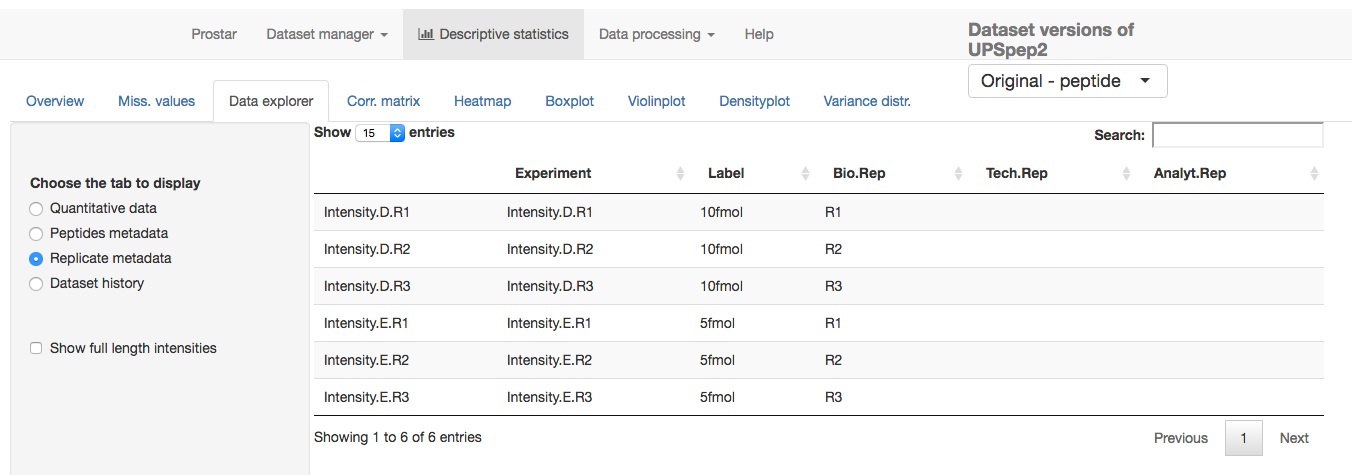
\includegraphics{images/desc_pdata.png}}
\caption{View of samples meta-data in the MSnSet dataset}\label{fig:sdqv3}
\end {figure}

The last tab, named "Dataset history" contains the log of the previous 
processing. Contrarily to the "Session log" panel (see 
Section~\ref{sec:sessionlog}), the information here does not relate to the 
session, and is saved from a session to the next one.

\hl{\bf Command line:}  The \Biocpkg{DAPAR} functions to get the three first 
tables are in fact those from the \Biocpkg{MSnbase} package: 
\Rfunction{exprs()} (Quantitative data), \Rfunction{fData()} 
(Analyte metadata) and \Rfunction{pData()} (Replicate metadata). 
% for \emph{Expression data}, \emph{Feature Meta Data} and 
%\emph{Samples Meta Data}.
Similarly, the "Dataset history" information is also accessible. In fact, 
it is stored in the slot (\Rcode{processingData}) of the current MSnSet 
object. In a R console, if \Rcode{obj} is the current dataset, it can be 
accessed by entering:
\begin{Schunk}
\begin{Sinput}
> getProcessingInfo(obj)
\end{Sinput}
\end{Schunk}
%% $

\subsubsection {Heatmap}
A heatmap is drawn with the associated dendrogram (see Fig.~\ref{fig:sdhm}). 
The colors represent the intensities: red for high intensities and green for 
low intensities. White color is reserved for missing values.
The dendrogram shows the hierarchical classification of the samples. This 
classification can be tuned by two parameters:
\begin {itemize}
\item \textbf{Distance}: Euclidean or Manhattan
\item \textbf{Linkage}: Ward.D or mean
\end {itemize}

\begin {figure}
\centering
\fbox{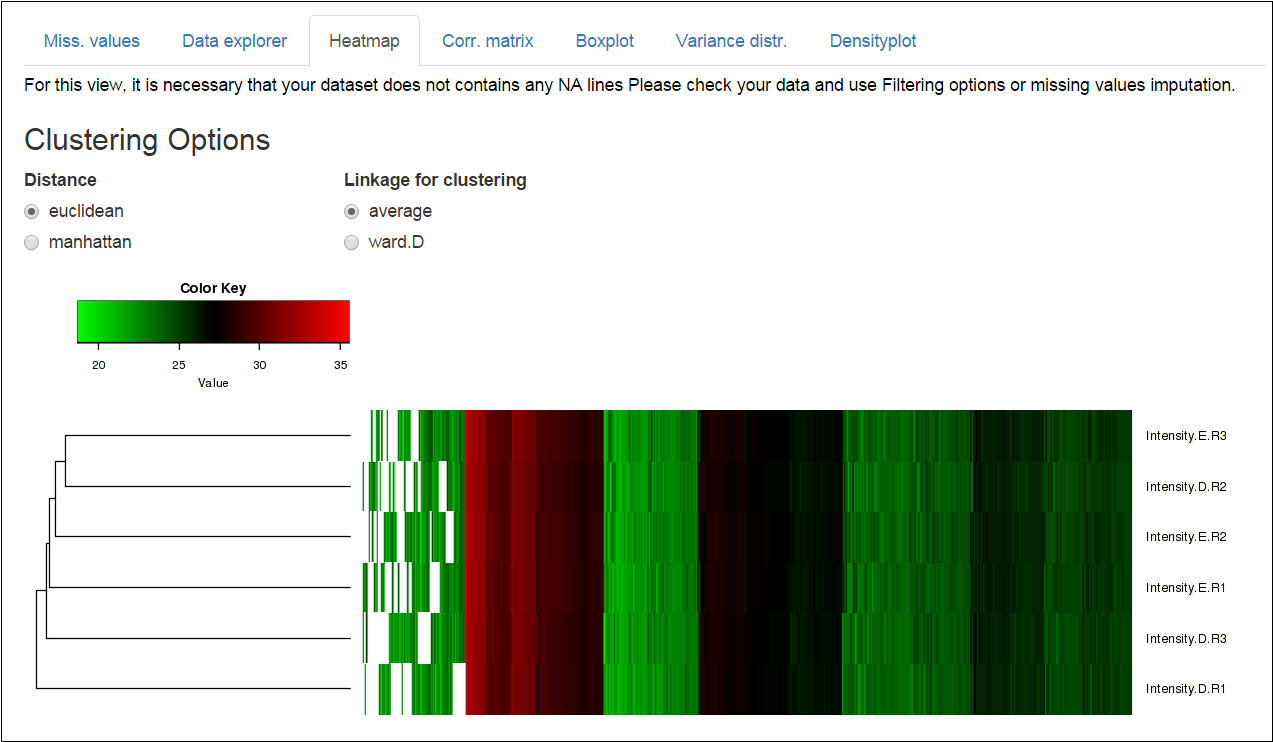
\includegraphics{images/desc_heatmap.png}}
\caption{Heatmap and dendrogram for the quantitative data.}\label{fig:sdhm}
\end {figure}

%%\hl{\bf Command line:} In \Biocpkg{DAPAR}, the corresponding function is 
%%\Rfunction{heatmapD()}.
\hl{\bf Command line:} In \Biocpkg{DAPAR}, the corresponding function are:
\begin{itemize}
\item for the dataframe parameter: \Rfunction{heatmapD()},
\item for an object of class MSnSet: \Rfunction{wrapper.heatmapD()}.
\end{itemize}

\subsubsection {Correlation matrix}

{In this tab, it is possible to visualize the extent to which the replicates 
correlate or not (see Fig.~\ref{fig:sdcm}). The contrast in the matrix may be 
changed by modifying the color gradient.}

\begin {figure}
\centering
\fbox{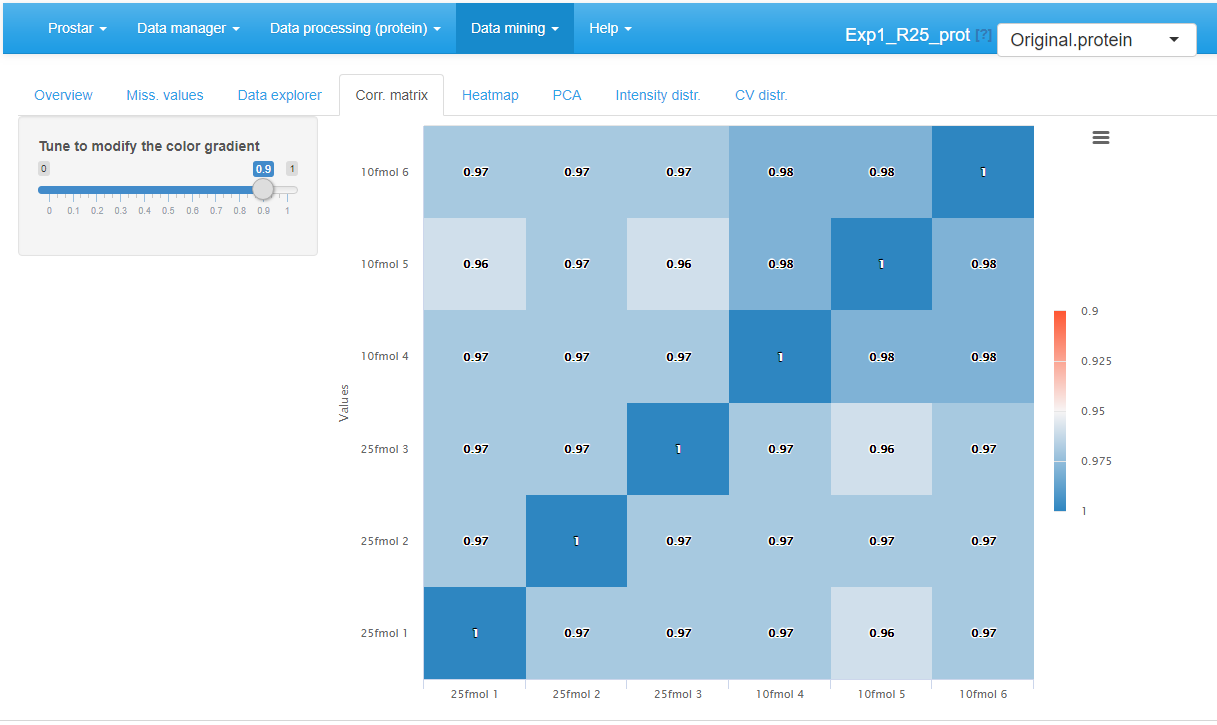
\includegraphics{images/desc_corrmatrix.png}}
\caption{Correlation matrix for the quantitative data.}\label{fig:sdcm}
\end {figure}

%%\hl{\bf Command line:} In \Biocpkg{DAPAR}, the corresponding function is 
%%\Rfunction{corrMatrixD()}.
\hl{\bf Command line:} In \Biocpkg{DAPAR}, the corresponding function are:
\begin{itemize}
\item for the dataframe parameter: \Rfunction{heatmapD()},
\item for an object of class MSnSet: \Rfunction{wrapper.heatmapD()}.
\end{itemize}


\subsubsection {Boxplot}\label{sec:boxplot}

The protein distribution by replicates is summarized with boxplots 
(see Fig.~\ref{fig:boxplot}). The user can change the legend of the samples 
(X-axis) by checking items in the checkboxes group. The colors of the boxes 
correspond to the different conditions (column \textbf{Label} in the table of 
\emph {Samples Meta Data}).

\begin {figure}
\centering
\fbox{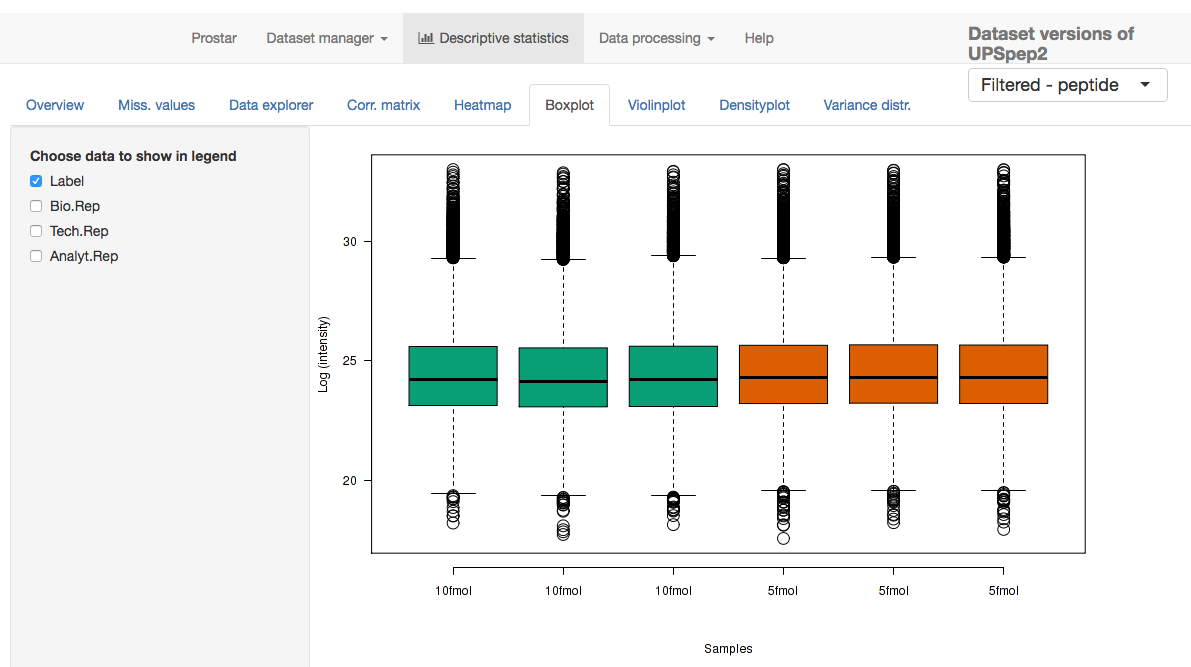
\includegraphics[width=0.6\textwidth]{images/desc_boxplot.png}}
\caption{Boxplot for the quantitative data.}\label{fig:boxplot}
\end {figure}



%%\hl{\bf Command line:} In \Biocpkg{DAPAR}, the corresponding function is 
%%\Rfunction{boxPlotD()}.
\hl{\bf Command line:} In \Biocpkg{DAPAR}, the corresponding functions are:
\begin{itemize}
\item for the dataframe parameter: \Rfunction{boxPlotD()},
\item for an object of class MSnSet: \Rfunction{wrapper.boxPlotD()}.
\end{itemize}



\subsubsection {Violin plot}\label{sec:violinplot}

The protein distribution by replicates is summarized with violin plots 
(see Fig.~\ref{fig:violinplot}). The user can change the legend of the samples 
(X-axis) by checking items in the checkboxes group. The colors of the boxes 
correspond to the different conditions (column \textbf{Label} in the table of 
\emph {Samples Meta Data}).

\begin {figure}
\centering
\fbox{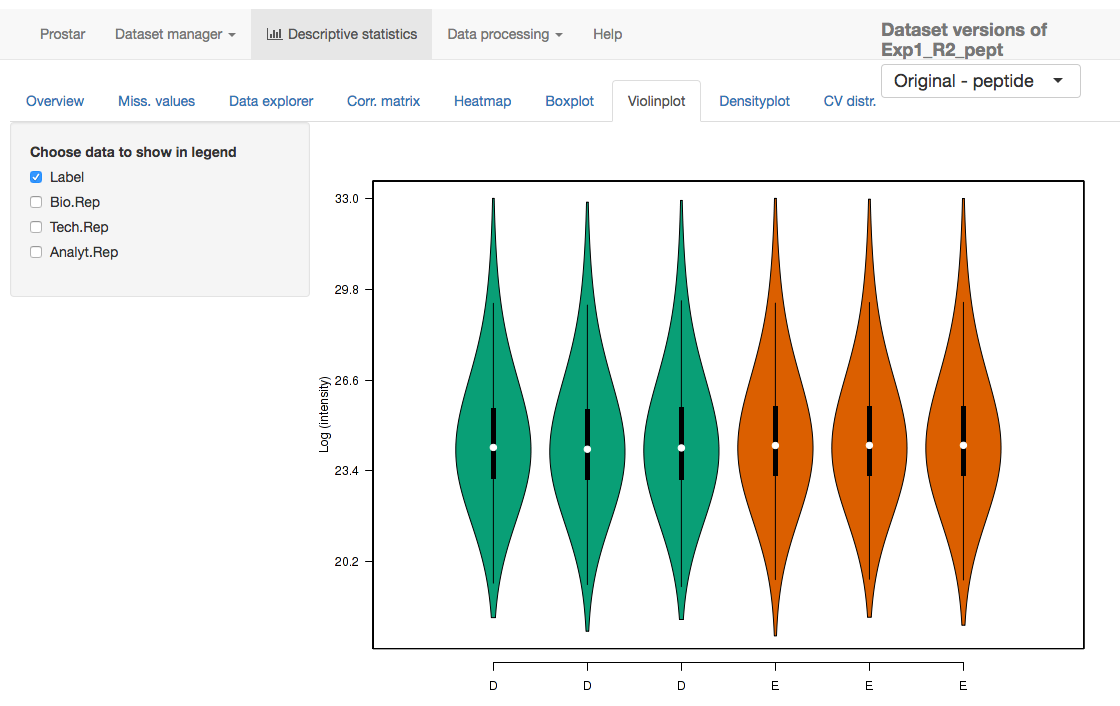
\includegraphics[width=0.6\textwidth]{images/desc_violinplot.png}}
\caption{Violin plot for the quantitative data.}\label{fig:violinplot}
\end {figure}



%%\hl{\bf Command line:} In \Biocpkg{DAPAR}, the corresponding function is 
%%\Rfunction{boxPlotD()}.
\hl{\bf Command line:} In \Biocpkg{DAPAR}, the corresponding functions are:
\begin{itemize}
\item for the dataframe parameter: \Rfunction{violinPlotD()},
\item for an object of class MSnSet: \Rfunction{wrapper.violinPlotD()}.
\end{itemize}



%%%%%%%%%%%%%%%%%%%%%%

\subsubsection{CV distribution}
This plot shows the distribution of the CV of the log-intensity of 
proteins for each condition (see Fig.~\ref{fig:sdvd}).

\begin {figure}
\centering
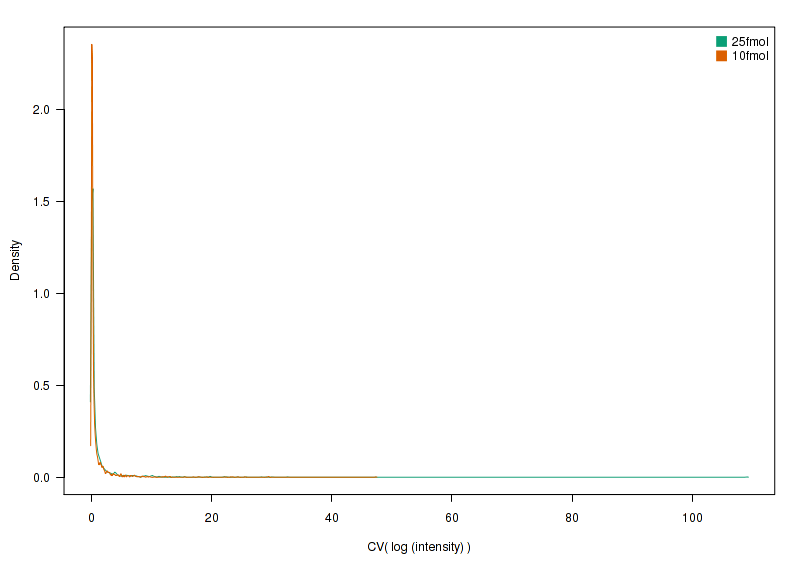
\includegraphics[width=0.75\textwidth]{images/desc_CVDist.png}
\caption{CV distribution for the quantitative data.}\label{fig:sdvd}
\end {figure}

\hl{\bf Command line:} In \Biocpkg{DAPAR}, the corresponding function is 
\Rfunction{varianceDistD()}.

\subsubsection{Density plot}\label{sec:densityplot}
This plots shows the distribution of the log-intensity of proteins for each 
condition (see Fig.~\ref{fig:sddp}).

\begin {figure}
\centering
\fbox{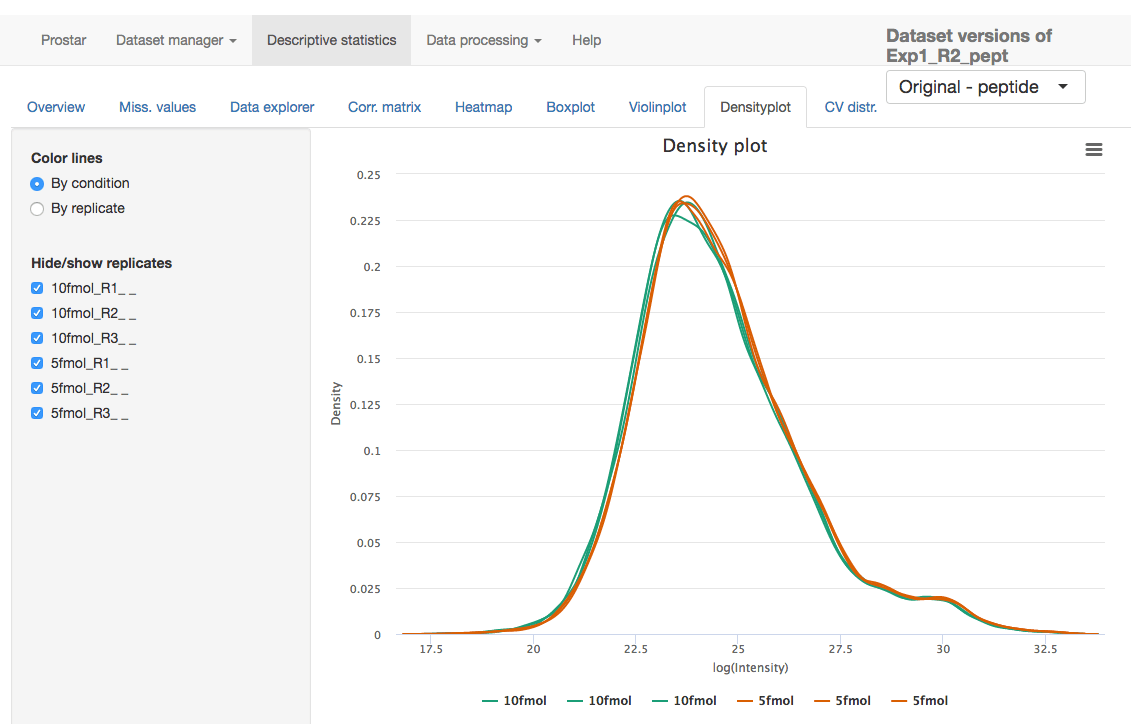
\includegraphics[width=0.67\textwidth]{images/desc_density.png}}
\caption{Densityplot the quantitative data.}\label{fig:sddp}
\end {figure}

{Two options are available to custom the plot:
\begin{itemize}
\item \textbf{Plot to show} which defines how to color the replicates: one 
color for each condition (value "By condition") or one color per replicate 
(value "By replicate"). By default, the data are colored by condition.
\item \textbf{Select data to show} Select the replicates to display. By 
default, all the replicates are showed.
\end {itemize}
}


%In \Biocpkg{DAPAR}, the corresponding function is \Rfunction{densityPlotD()}.
\hl{\bf Command line:} In \Biocpkg{DAPAR}, the corresponding functions are:
\begin{itemize}
\item for the dataframe parameter: \Rfunction{densityPlotD()},
\item for an object of class MSnSet: \Rfunction{wrapper.densityPlotD()}.
\end{itemize}


%%%%%%%%%%%%%%%%%%%%%%%%%%%%%%%%%%%%%%%%%%%
%% Menu
%%%%%%%%%%%%%%%%%%%%%%%%%%%%%%%%%%%%%%%%%%%
\subsection{Data processing}\label{sec:processingadataset}

The "Data processing" menu contains the 5 predefined steps of a quantitative 
analysis. They are designed to be used in a specific order:
\begin{enumerate}
\item {Filtering}
\item{Normalization}
\item{Missing values imputation}
\item{Aggregation}
\item{Differential analysis}
\end{enumerate}
For each step, several algorithms or parameters are available, and they are 
toroughly detailled in the sequel of this section.

During each of these 5 steps, it is possible to test several options, and to 
observe the influence of the processing in the descriptive statistics menu 
(see Section~\ref{sec:descriptivestatistics}), which is dynamically updated. 

Finally, once the ultimate tuning is chosen for a given step, it is advised 
to save the processing. By doing so, another dataset appears in the "Dataset 
versions" list (see Section~\ref{sec:availabledatasets}). Thus, it is possible 
to go back to any previous step of the analysis if necessary, without starting 
back the analysis from scratch.

%%%%%%%%%%%%%%%%%%%%%%%%%%%%
\subsubsection{Filtering}\label{sec:filtering}
{In this step, the user may decide to delete several peptides or proteins 
according to several criteria:
If the amount of missing values is too important to expect confident 
processing (Tab 1); or if they are identified as reverse sequences (for 
target-decoy approaches) or contaminants (Tab 2).}
%This tool allows the user to deal with missing values in quantitative data 
%by deleting lines that contain a certain amount of quantitative values. 

\begin {figure}
\centering
\fbox{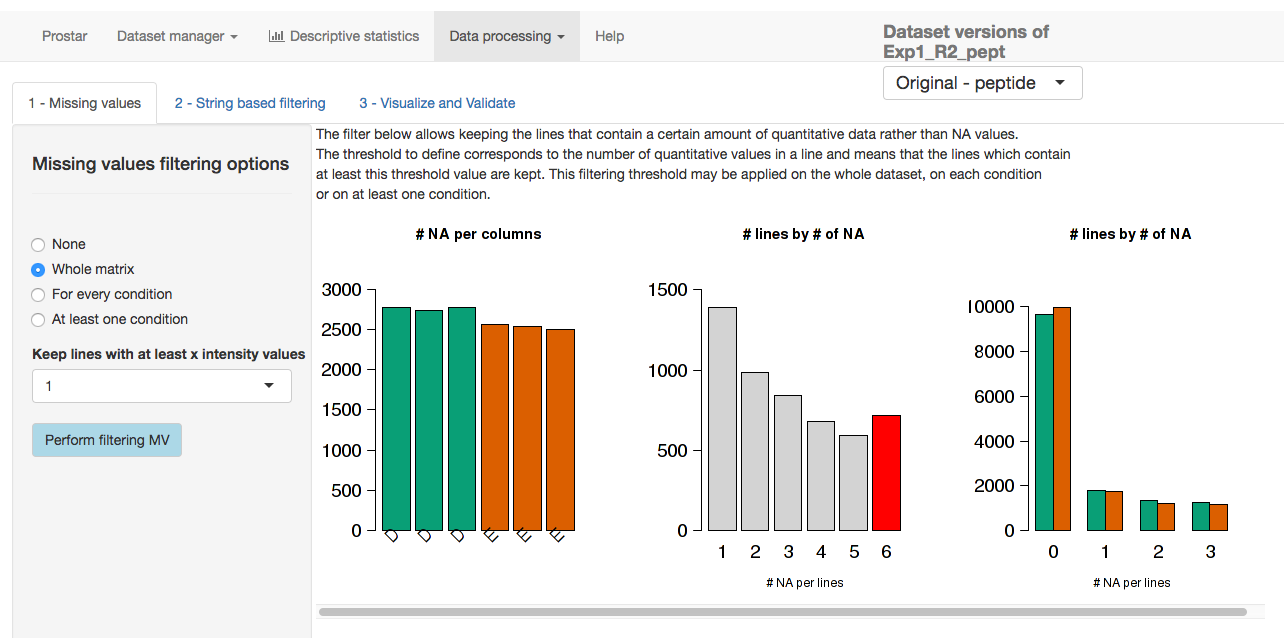
\includegraphics[width=\textwidth]{images/filter1.png}}
\caption{Interface of the filtering tool - 1.}\label{fig:filter1}
\end {figure}

\begin {figure}
\centering
\fbox{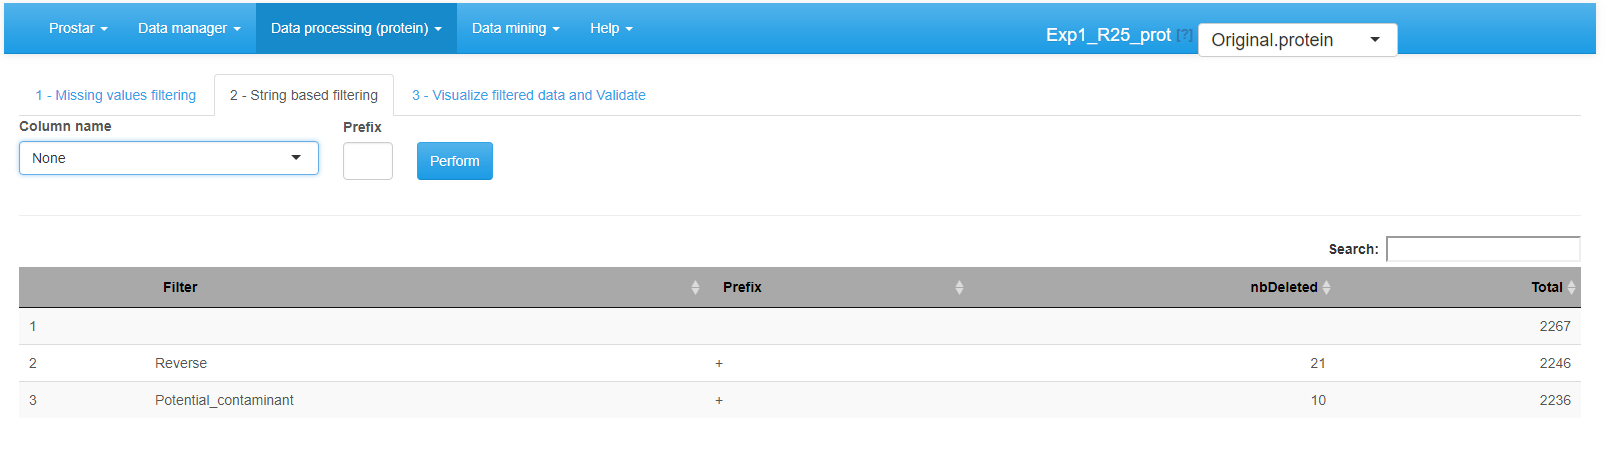
\includegraphics[width=\textwidth]{images/filter2.png}}
\caption{Interface of the filtering tool - 2.}\label{fig:filter2}
\end {figure}

\begin {figure}
\centering
\fbox{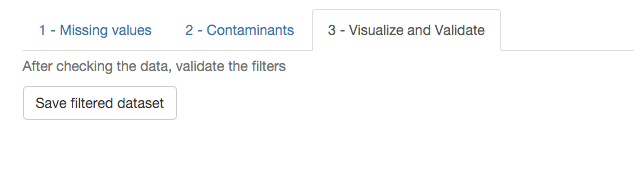
\includegraphics[width=\textwidth]{images/filter3.png}}
\caption{Interface of the filtering tool - 3.}\label{fig:filter3}
\end {figure}

To filter the missing values (first tab called "Missing values"), the choice 
of the lines to be deleted is made by different options (see 
Fig.~\ref{fig:filter1}):
\begin {itemize}
\item\textbf{None}: No filtering, the quantitative data is left unchanged. 
This is the default option;
\item\textbf{Whole Matrix}: The lines (across all conditions) in the 
quantitative dataset which contain less non-missing value than a 
user-defined threshold are deleted;
\item\textbf{For every condition}: The lines for which each condition 
contain less non-missing value than a user-defined threshold are deleted;
\item\textbf{At least one condition}: The lines for which at least one 
condition contain less non-missing value than a user-defined threshold 
are deleted;
\end {itemize}

The user can visualize the effect of filter options without changing the 
current dataset by clicking on "Perform filtering". If the filtering does not 
produce the expected effect, the user can test another one. To do so, one 
simply has to choose another method in the list and click again on "Perform 
filtering". The plots are automatically updated. This action does not modify 
the dataset but offers a preview of the filtered data. The user can visualize 
as many times he/she wants several filtering options. 

Afterwards, the user can choose to remove contaminants and reverses in the 
second tab called "String based filtering". To do so, he/she selects the 
appropriate columns of the metadata listed in the dropdown menus. Then, 
he/she specifies in each of these columns the prefix chain of characters 
that identifies the analytes to filter.

\textbf{Remark:} If he/she has no idea of the prefixes, he/she can switch to 
the Data Explorer in the Descriptive Statistics menu, so as to visualize the 
corresponding metadata. 

For each fullfilled option, the barplot below is updated: it shows the 
proportion of quantitative data, contaminants and reverses. Once the choices 
are made, the user click on "Perform string based filtering" to remove 
corresponding lines.

{Once the filtering is appropriately tuned, the user goes to the last tab 
(called "visualize and Validate") (see Fig.~\ref{fig:filter3}), to visualize 
the set of analytes that have been previously filtered. On the left panel, 
one chooses among the lines filtered on missing values, contaminants or 
reverse; Then, the corresponding data table is diplayed on the right panel. 
Finally, one clicks on "Apply filter" so as to validate the user's choice and 
to apply it to the dataset. The information related to the type of filtering 
as well as to the chosen options appears in the Session log tab (see 
Section~\ref{sec:sessionlog}). A new dataset is created; it becomes the new 
current dataset and its name appears in the \textbf{Dataset versions} menu at 
the top of the screen. All plots and tables available in \Biocpkg{ProStaR} 
are automatically updated.}

%\textcolor{red}{At this time, there is no version that works directly on 
%dataframes.}
\hl{\bf Command line:} In \Biocpkg{DAPAR}, the function to filter missing 
values is \Rfunction{mvFilter()}. The other types of filters corresponds to 
classical data structure manipulation with R.


%%%%%%%%%%%%%%%%%%%%%%%%%%%%
\subsubsection{Normalization}\label{sec:normalization}

The next step is to normalize the replicates so as to have more accurate 
comparisons. \Biocpkg{ProStaR} offers a number of different normalization 
routines that are described below.

In order to visualize the data after normalization, three plots are displayed:
a boxplot, a plot that displays the differences between data before and after 
the normalization and a densityplot (see Fig.~\ref{fig:norma}). The first and 
the third plots are the same as the one showed in \textbf{Descriptive 
Statistics}, thus they have the same options (see 
Sections~\ref{sec:boxplot}~and~\ref{sec:densityplot}).

\begin {figure}
\centering
\fbox{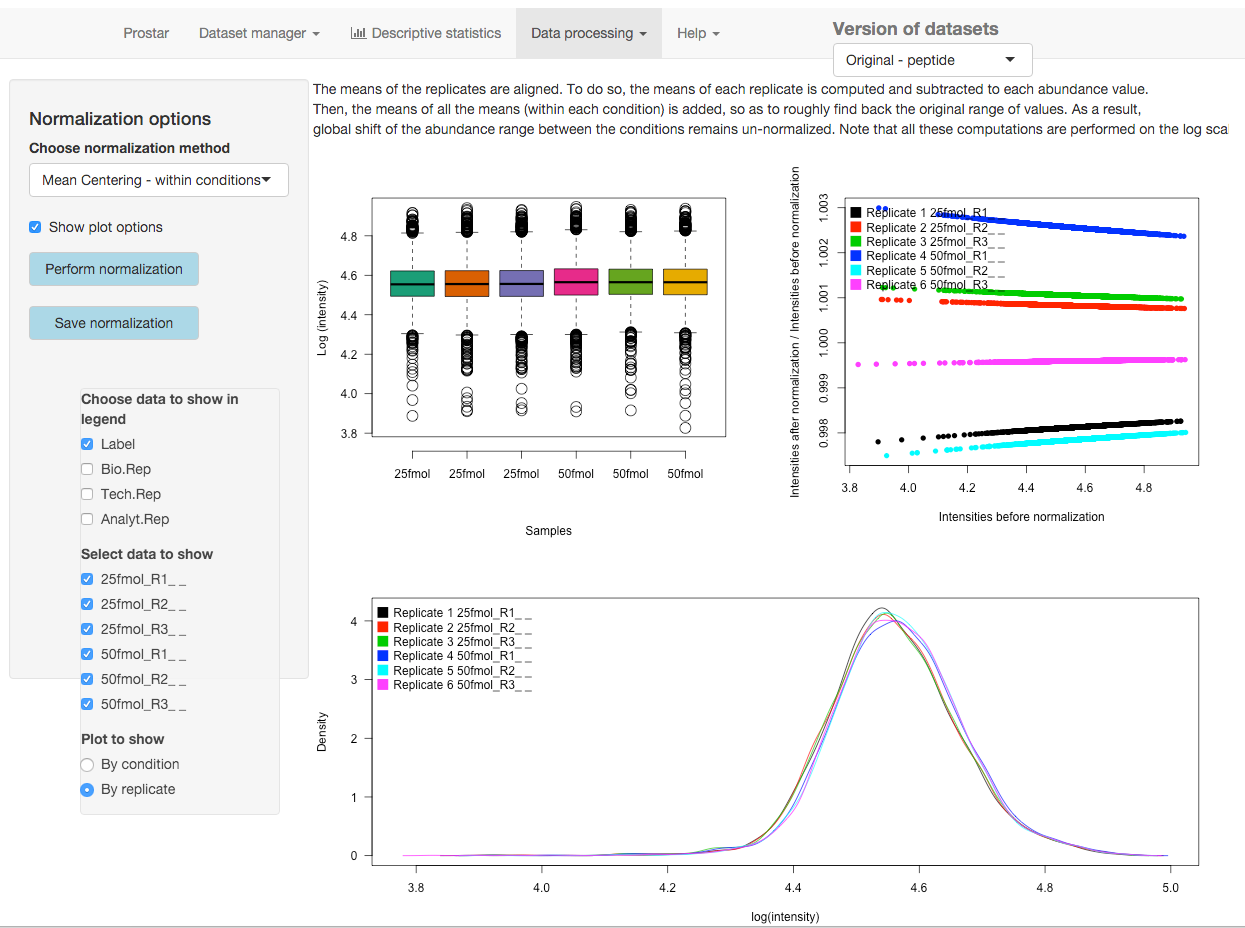
\includegraphics[width=\textwidth]{images/normalisation.png}}
\caption{Interface of the normalization tool.}\label{fig:norma}
\end {figure}

If no normalization is necessary, it is possible to skip this step.
If the user wants to compare the influence of several normalization methods, 
it is possible to select them in a row, and to alternate between this menu 
and the "Descriptive statistics" one. It is possible to go back to the 
original dataset by selecting "None".
%They are grouped into two families: "global adjustments" and adjustments 
%by centering:
Several methods are implemented:
\begin {description}
%  \item \textbf{Global adjustment}:
%    \begin {itemize}
\item[Global alignment]
These methods propose normalizations of important magnitude that should be 
cautiously used:
\begin{itemize}
\item \textbf{sum by columns} operates on the original scale (not the log2 one) 
and propose to normalize each abundance by the total abundance of the sample 
(so as to focus on the analyte proportions among each sample).
\item \textbf{quantile alignment} proposes to align the quantiles of all the 
replicates as described in [ref1]; practically it amounts to replace abundances 
by order statistics.\newline
\end{itemize}


\item[Quantile centering]
These methods propose to shift the sample distributions (either all of them at 
once, or within each condition at a time) to align a specific quantile: the 
median (under the assumption that up-regulations and down-regulations are 
equally frequent), the 15 quantile (under the assumption that the signal/noise 
ratio is roughly the same in all the samples), or any other user's choice. 
Two parameters are available:
\begin{itemize}
\item \textbf{Normalization type: } the centering can operate over the entire 
dataset (value "overall") or over each condition (value "within conditions"),
\item \textbf{Value of quantile (in \%): } 0.15 (lower limit/noise), 
0.5 (median) or Other (In that case, the user can choose its own quantile 
value).\newline
\end{itemize}


\item[Mean centering]
These methods propose to shift the sample distributions (either all of them at 
once, or within each condition at a time) to align their means. It is also 
possible to force unit variance (or not). Two parameters are available:
\begin{itemize}
\item \textbf{Normalization type:} the centering can operate over the entire 
dataset (value "overall") or over each condition (value "within conditions"),
\item \textbf{Include variance reduction:} Let the user choose if he/she wants 
to rescale the dataset to have unitary variance.
\end{itemize}

    % \item[Sum by column] The abundance of each protein is divided by the 
    % total abundance of all the proteins in the same replicates. This 
    % normalization is interesting to compare the proportions of a given 
    % protein in different samples that do not necessarily contain the same 
    % amount of biological material. Contrarily to the others, this 
    % normalization is not performed on the log2 scale, for it would not have 
    % any interpretation (the data are thus exponentiated and 
    % re-log2-transformed as pre-and post-processing).
    % \item[Quantiles] The protein abundance are roughly replaced by the order 
    % statics on their abundance (from package \Biocpkg{preprocessCore}). This 
    % is the strongest normalization method available, and it should be use 
    % carefully, for it erazes most of the difference between the samples.
%    \end {itemize}
%  \item \textbf {Adjustment by centering}:
%  \begin {itemize}
%     \item[Mean / median centering] The central tendancies of the samples 
%     are aligned. To do so, one computes first the central tendancy (either 
%     the mean of the median, depending on the user choice) for each replicates.
%     Then, to each abundance value, one subtracts the corresponding central 
%     tendancy. Finally, one adds to this abundance value, an offset in order 
%     to find roughly back the original range of values. Depending on the 
%     user's choice, this offset can be the mean of all the central tendancies, 
%     whatever the conditions (then, any global difference between the 
%     conditions will disappear);  or it can be the mean of all the central 
%     tendancies within each conditions (then, any global difference between 
%     the conditions is preserved).
% Note that all these computations are performed on values that were originaly 
% log2-transformed.
%     \item[Mean centering and scaling] The spirit of this normalization is 
%     the same as the previous one, yet, it is stronger, and it only applies 
%     to log2-tranformed abundance values that distributes roughly normaly for 
%     each sample. Basically, a mean centering as described above is applied. 
%     Then, the variance of the distribution is re-scaled to 1. Let us note 
%     that median centering is not really adapted to a rescaling the variance; 
%     this is why such combination of parameters is not available. Once again, 
%     the centering can operate over the entire dataset, or over each condition.
%     on all conditions,
%     \item Centering over median on each condition,
%     \item Centering over mean on all conditions,
%     \item Centering over mean on each condition,
%     \end {itemize}
% %    \item \textbf {Adjustment by centering}
%     \begin {itemize}
%     \item Centering and reduction by mean and standard deviation.
%     \end {itemize}
\end {description}

Each time the user selects a method, the explanation above is displayed. The 
user can visualize the effect of a normalization method without changing the 
current dataset. If the normalization does not produce the expected effect, 
the user can test another one. To do so, one simply has to choose another 
method in the list and click on "Perform normalization". The plots are 
automatically updated. This action does not modify the dataset but offers a 
preview of the normalized quantitative data.
The user can visualize as many times he/she wants several normalization 
methods. Once he finds the correct one, he/she validates his/her choice by 
clicking on "Save normalization". Then, a new "normalized" dataset is created 
and loaded in memory. The method of normalization that has been used is 
added to the Session log tab (see section~\ref{sec:sessionlog}). It becomes 
the new current dataset and the name "Normalized" appears in "Dataset 
versions". All plots and tables in other menus are automatically updated.

%\hl{\bf Command line:} In \Biocpkg{DAPAR}, the corresponding function is 
%%\Rfunction{normalizeD()}.
{\hl{\bf Command line:} In \Biocpkg{DAPAR}, the functions for the plot 
"before-after normalization" are:
\begin{itemize}
\item for the dataframe parameter: \Rfunction{compareNormalizationD()} ,
\item for an object of class MSnSet: 
\Rfunction{wrapper.compareNormalizationD()} .
\end{itemize}}


The corresponding functions for the normalization are:
\begin{itemize}
\item for the dataframe parameter: \Rfunction{normalizeD()},
\item for an object of class MSnSet: \Rfunction{wrapper.normalizeD()}.
\end{itemize}

\subsubsection{Imputation}\label{imputation}

Two plots are available in order to help the user choose the right 
imputation method for his dataset (see Fig.~\ref{fig:impu}).


The scatter plot on the left hand side displays the proteins in a space 
spanned by the mean abundance ($x$ axis) and the number of missing values 
($y$ axis). Note that for each protein, as many points (of different colors) 
as conditions are displayed, for each condition is processed independently of 
the others. As a result, the maximum value on the $y$ axis is given by the 
number of replicates in a condition (depending on the filtering step). Let 
us note that the points have been slightly jittered on the $y$ axis to 
enhance a better visualization.

%shows the distribution of the mean of intensity of proteins (X-axis) in 
%function of the number of missing values contained in the line (Y-axis) of 
%the corresponding protein. The different conditions are colored by different 
%colors. The points in the Y-axis have been jittered to an easier view.
This plot indicates how the missing values are distributed over the range of 
intensity: if there are lots of missing values in the low intensity region 
(indicating a censoring mechanism produced the missing values) or if they are 
uniformly distributed. 
%In the first case, that means the missing values are likely MNAR and in the 
%second case, they might be MCAR.


The heatmap on the right hand side clusters the proteins according to their 
distribution of missing values across the conditions. Each line of the map 
depicts a protein. On the contrary, the columns do not depicts the replicates 
anymore, as the abundance values have been reordered so as to cluster the 
missing values together. Similarly, the proteins have been reordered, so as 
to cluster the proteins that have a similar amount of missing values 
distributed in the same way over the conditions. Each line is colored so as 
to depicts the mean abundance value within each condition. This heatmap is 
also helpful to decide what is the main origin of missing values (random 
missingness or censoring of the low intensities).


\begin {figure}
\centering
\fbox{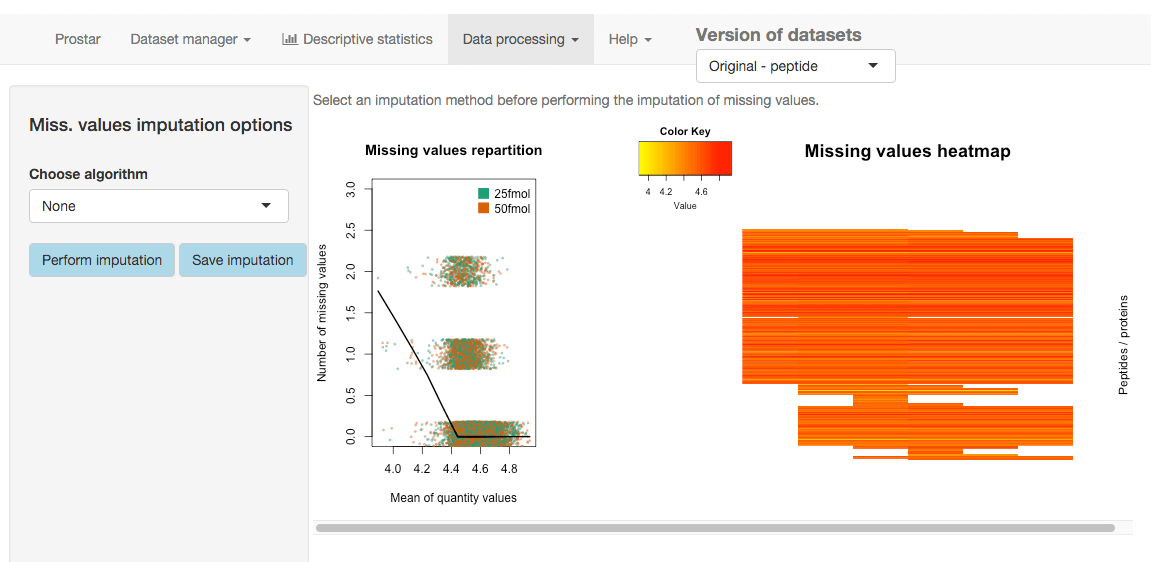
\includegraphics[width=\textwidth]{images/imputation.png}}
\caption{Interface of the imputation of missing values tool.}\label{fig:impu}
\end {figure}

\textcolor{red}{
The user can choose one of the several available imputation methods, depending 
on the type of missing values:
\begin{itemize}
\item If the missing values are due to a mixture of censorship and of randomness
, it is advised to use the functions of the package \CRANpkg{imp4p}. This 
package is a collection of proteomic-specific 
multiple imputation methods that operate on peptide-level datasets and which 
propose to impute each missing value according to its nature (censored or 
random). Two parameters are available: the number of iterations (the more 
iterations, the more accurate the results, yet the more time-consuming) and a 
checkbox to let the user choose if he/she wants to impute the LAPALA. This
term coined from French "là/pas-là"(meaning "here/not-here") refers to analytes 
(peptides or proteins) that are entirely missing in some conditions while they
are (partially or totally) visible in others. Their specific accounting in a 
conservative way is a real issue as the imputation cannot rely on any observed 
value in a given condition. The parameter "Upper LAPALA bound" defines the 
maximum imputed value as a centile of the observed distribution (a tuning 
between 0\% and 10\% is advised). 
\item Alternatively, it is possible to use KNN ($K$ Nearest Neighbors) from package 
\Biocpkg{impute} or MLE (Maximum Likelihood Estimation) from package 
\Biocpkg{norm}.
\end{itemize}
}

The user can visualize the effect of an imputation method without changing 
the current dataset. If the imputation does not produce the expected effect, 
the user can test another one. To do so, one simply has to choose another 
method in the list and click on "Perform imputation". The plots are 
automatically updated. This action does not modify the dataset but offers a 
preview of the imputed quantitative data.
The user can visualize as many times he/she wants several imputation methods. 
Once he finds the correct one, he/she validates his/her choice by clicking on 
"Save imputation". Then, a new "imputed" dataset is created and loaded in 
memory. The method of imputation used is added to the Session log tab (see 
Section~\ref{sec:sessionlog}). This new dataset becomes the new current 
dataset and the name "Imputed" appears in "Dataset versions". All plots and 
tables in other menus are automatically updated.

{\hl{\bf Command line:} In \Biocpkg{DAPAR}, the function used to impute the 
missing values is \Rfunction{mvImputation()}. The two aforementioned plots 
are obtained with respectively:
\begin{itemize}
\item for the dataframe parameter: \Rfunction{mvTypePlot()} and 
\Rfunction{mvImage()},
\item for an object of class MSnSet: \Rfunction{wrapper.mvTypePlot()} and 
\Rfunction{wrapper.mvImage()}.
\end{itemize}}

%%%%%%%%%%%%%%%%%%%%%%%%%%%%%%
\subsubsection{Aggregation}\label{aggregation}


{When working on a protein dataset, this step should be bypassed. On the other 
hand, when working on peptide datasets, one may want to conduct the 
differential analysis at protein level, for proteins are the biological units 
of interest. To do so, it is necessary to estimate the abundance of the 
proteins on the basis of those of the peptides. This is what the Aggregation 
step is made for.}

{First, the user chooses the "protein id" of the dataset, i.e. the column in 
the metadata, that contains the IDs of all the parent proteins for each 
peptide. 
Two barplots show up (Fig.~\ref{fig:agreg1} ). They provide the distribution 
of proteins according to their number of peptides (either all of them, or 
only those which are specific to a single protein). These statistics are 
helpful to visualize the adjacency matrix of the peptide-protein graph, that 
is sometime rather big.}


\begin {figure}
\centering
\fbox{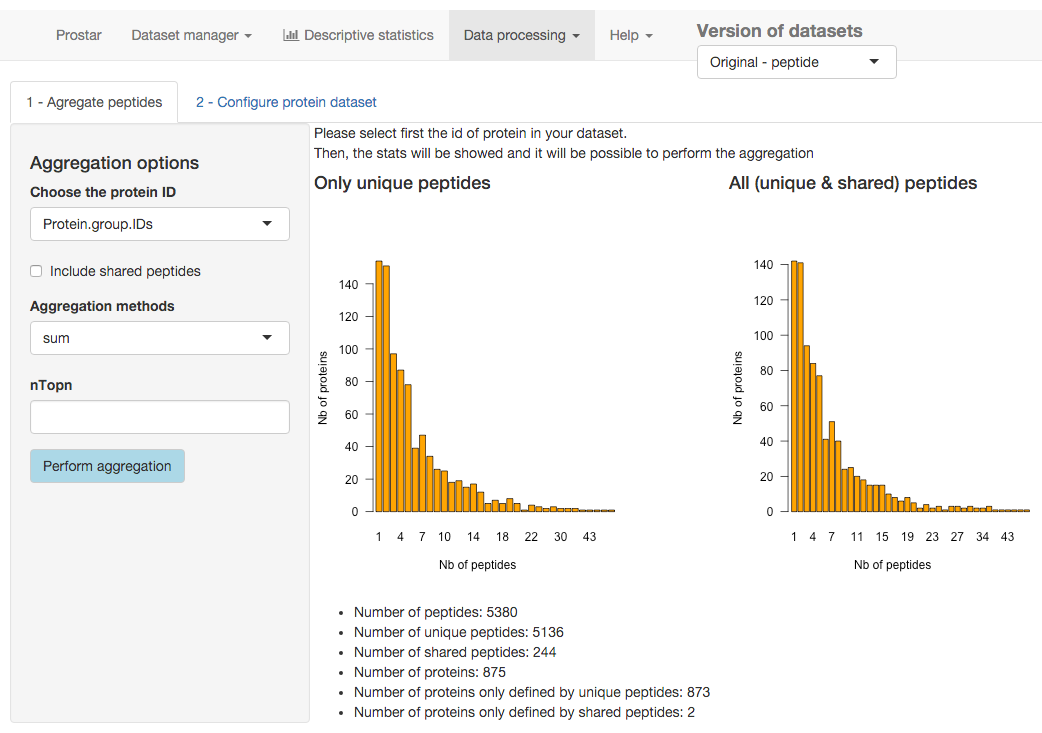
\includegraphics[width=\textwidth]{images/agregation1.png}}
\caption{Interface of the agregation tool - 1.}\label{fig:agreg1}
\end {figure}

\begin {figure}
\centering
\fbox{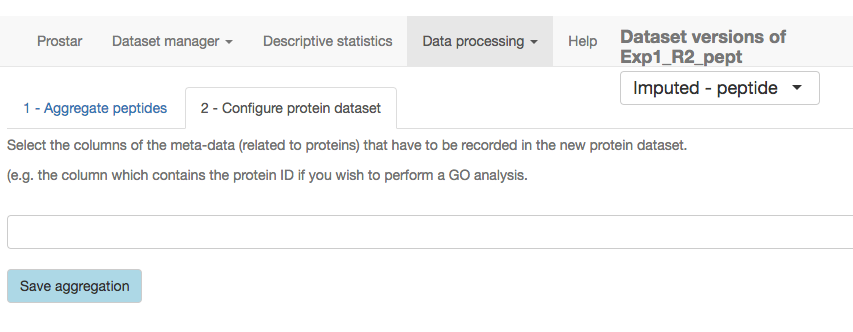
\includegraphics[width=\textwidth]{images/agregation2.png}}
\caption{Interface of the agregation tool - 2.}\label{fig:agreg2}
\end {figure}


Second, a checkbox is used to indicate whether the user wants the shared 
peptides to be accounted for during the aggregation process.

Third, the aggregation method itself ust be chosen: 
\begin{itemize}
\item Sum: that is the sum of the peptide intensities,
\item Mean: the mean of the peptide intensities,
\item Sum on top n: that is the sum over the N peptides with the highest median 
intensities - in this case, the additional parameter N must be tuned.
\end{itemize}

On the next tab, the user selects the columns of the peptide dataset that 
are of interest to be kept in the metadata of the protein dataset (e.g. the 
sequence of the peptides). The effect of this action is to compile, for a 
given parent-protein, the information of all of its child-peptides, and to 
store them in a dedicated column. Once done, one validates the user's choice 
by clicking on "Save aggregation". Then, a new "aggregated" dataset is 
created and loaded in memory. The aggregation method that was finally used is 
recorded in the Session log tab (see section~\ref{sec:sessionlog}). This new 
dataset becomes the new current dataset and the name "Aggregated" appears in 
"Dataset versions". All plots and tables in other menus are automatically 
updated.

The aggregation being more computationaly demanding than other processing 
steps, the current version of \Biocpkg{ProStaR} does not provide the same 
flexibility regarding the parameter tuning: Here, it is necessary to save the 
aggregation result first, then, to go to "descriptive statistics" to check 
the results, and possibly to go back to the imputed dataset with the "Dataset 
versions" dropdown menu to test another aggregation tuning. Contrarily to 
other processing steps, it is not possible to visualize on-the-fly the 
consequences of the parameter tuning, and to save it afterwards. We are 
currently working on improving this issue for the next versions 
of \Biocpkg{ProStaR}. 
%The user can visualize  the effect of any aggregation method without changing 
%the current dataset. If the aggregation does not produce the expected effect, 
%the user can test another one. To do so, one simply has to choose another 
%method in the list and click on "Perform aggregation". The plot is 
%automatically updated. This action does not modify the dataset but offers a 
%preview of the aggregated data. The user can visualize  as many times he/she 
%wants several aggregation methods. Once he finds the correct one, he/she can 
%switch to the next tab called "Configure protein dataset".

Naturally, the output of this step is not a peptide dataset anymore, but a 
protein dataset. As a result, all the plots available in \Biocpkg{ProStaR} 
are deeply modified. For instance, the barplots summarising the 
peptide-protein graphs disapear because they have become meaningless.



\hl{\bf Command line:} In \Biocpkg{DAPAR}, the function used to compute the 
adjacency matrix peptides-proteins is \Rfunction{BuildAdjacencyMatrix()} and 
the one used to agregate the peptides into proteins is 
\Rfunction{AggregatePeptides()}. The aforementioned plot is obtained with the 
functions \Rfunction{GraphPepProt()}.



%%%%%%%%%%%%%%%%%%%%%%%%%%%%%%%%%%%%%%%%%%%%%%%%%%%%%%%%
\subsubsection{Differential analysis}\label{diffana}

This step cannot be conducted if the dataset still contains some missing 
values: They must be imputed before.
%In the case of mising values, the user have to proceed to the imputation 
%before the differential analysis.

{The differential analysis is divided into four steps, each impersonated by a 
different tab:
\begin{itemize}
\item Volcano plot,
\item $p$-value calibration,
\item FDR,
\item Validate \& save.
\end{itemize}}


\textbf {Volcano plot} (see Fig.~\ref{fig:anadiff1}): It is a scatter plot 
where each analyte is represented by 2 coordinates, namely a $p$-value on the 
Y-axis (more precisely -log10($p$-value)) and a fold change (FC) on the 
X-axis. Regarding the computation of the $p$-values, two tests are available 
in \Biocpkg{DAPAR}, depending on the user's choice: the Welch $t$-test 
(from package \CRANpkg{stats}) and the moderated $t$-test (from package 
\Biocpkg{limma}).
As an option, it is possible to redefined the sets of conditions that are 
tested one against the other. 
Then, the $p$-values are computed and a volcanoplot is displayed. 
%It shows on the $x$ axis the Fold Change (FC) between the two conditions, 
%and on the $y$ axis, . 
Finally, the user can tune a threshold on the FC. It allows discriminating 
some analytes for which the difference of expression between the condition is 
not important enough to be biologically relevant.

This is an interactive plot which reacts to mouse's events :
\begin{itemize}
\item When the user puts the pointer of his mouse over a
point of the plot, a tooltip window appears and shows some informations about 
that point. He can select the items to show in the Select widget where the 
different choices correspond to the columns of the feature meta-data table. 
The tooltip window is automatically updated,
\item When the user clicks on a point, a table is displayed above the 
volcanoplot. It shows the values of intensities for all the samples related to
the selected point. The cells colored in blue indicate that the corresponding 
value was a missing value in the original dataset and has been imputed,
\item The user can click and draw a rectangle on the plot to zoom in. 
By clicking on the button named "Reset zoom", the user can return to the 
entire plot.
\end{itemize}

\begin {figure}
\centering
\fbox{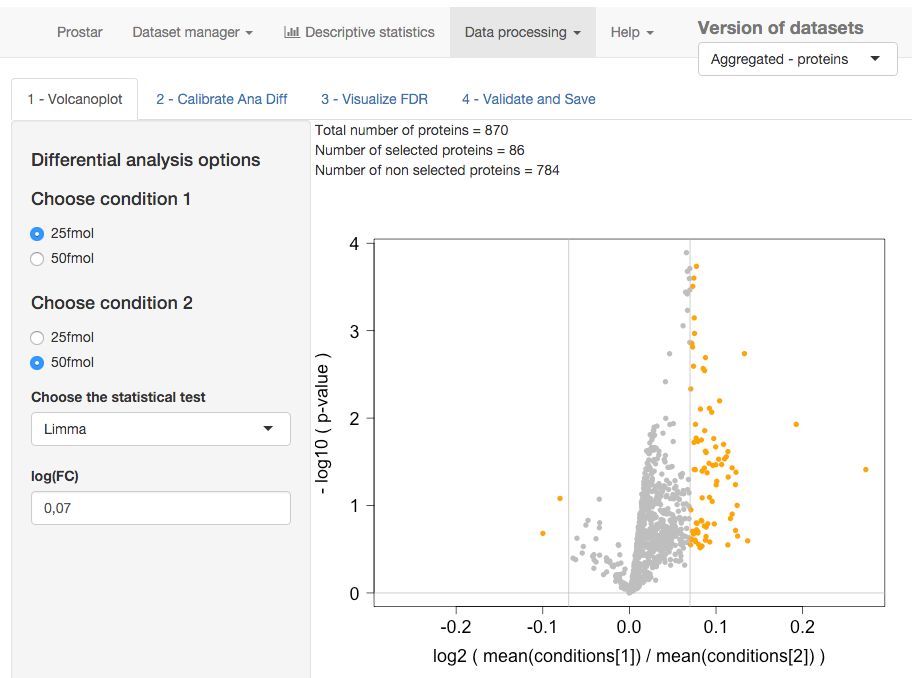
\includegraphics[width=0.6\textwidth]{images/anaDiff1.png}}
\caption{Volcanoplot of the differential analysis tool - 1.}
\label{fig:anadiff1}
\end {figure}


\textbf{$p$-value calibration (see Fig.~\ref{fig:anadiff2})}: In this tab, 
the fonctionalities of \CRANpkg{CP4P} have been wrapped. Future versions of 
\Biocpkg{ProStaR} will propose a more refined integration. To date, we 
redirect the reader to the \CRANpkg{CP4P} tutorial: 
\url{https://sites.google.com/site/thomasburgerswebpage/download/tutorial-CP4P-
4.pdf?attredirects=0}. 

\begin {figure}
\centering
\fbox{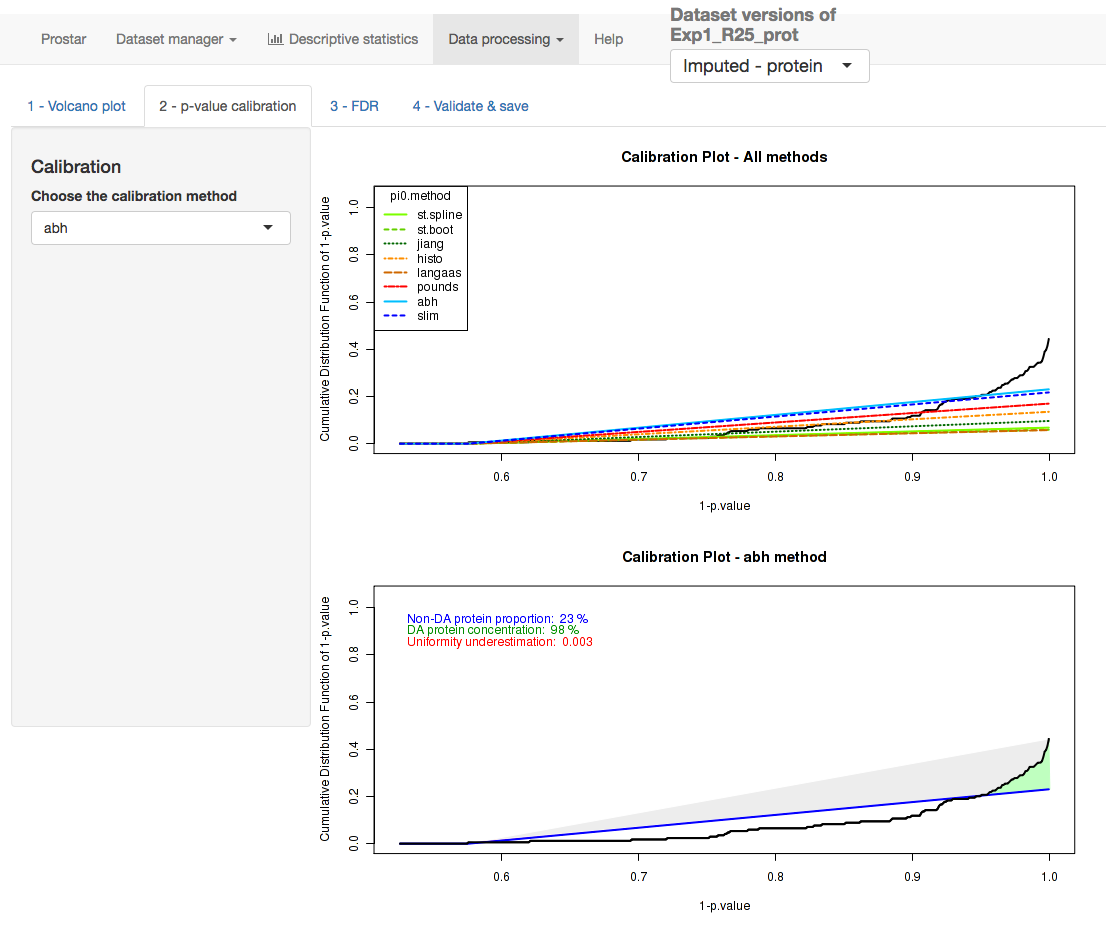
\includegraphics[width=0.6\textwidth]{images/anaDiff2.png}}
\caption{Calibration plot of the differential analysis tool - 2.}
\label{fig:anadiff2}
\end {figure}


\begin {figure}
\centering
\fbox{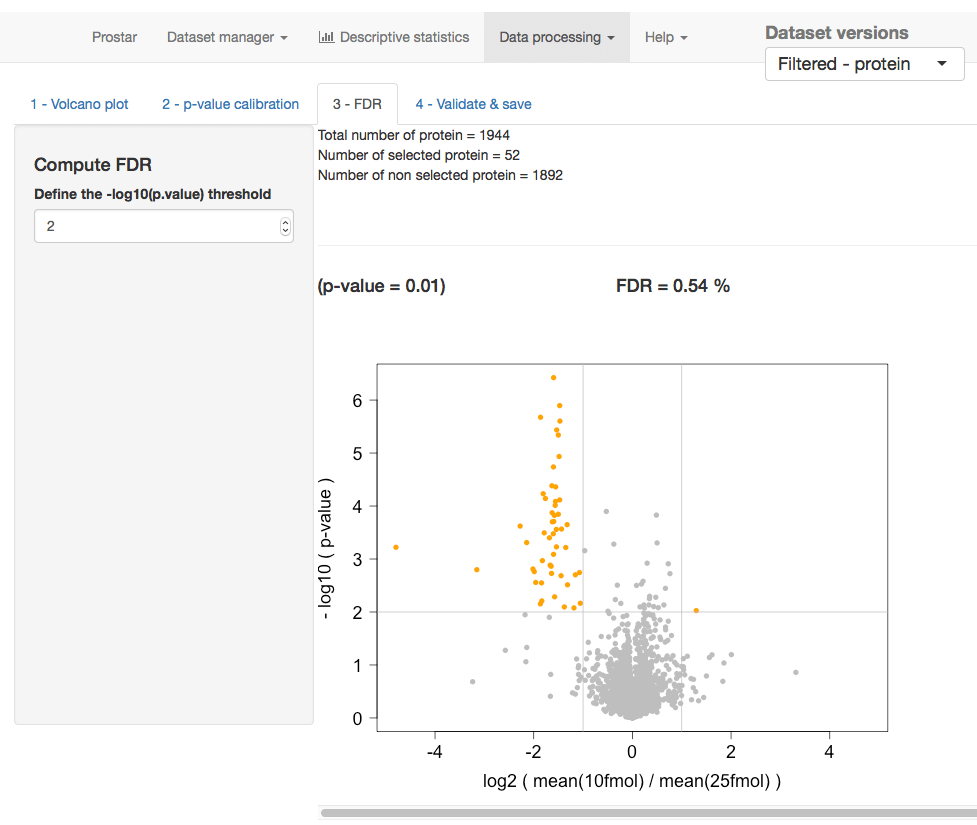
\includegraphics[width=0.6\textwidth]{images/anaDiff3.png}}
\caption{p-Value threshold of the differential analysis tool - 3.}
\label{fig:anadiff3}
\end {figure}

\textbf{FDR} (see Fig.~\ref{fig:anadiff3}): This tab also displays the 
volcano plot. A threshold along the $p$-value axis can be tuned by the user, 
so as to discriminate the differentially abondant proteins (which are 
highlighted). A horizontal straight line is drawn to visualize the threshold. 
The corresponding FDR is computed. The user can adjust the thresholds in 
order to select the maximum of proteins by minimizing the FDR.


\hl{\bf Command line:} In \Biocpkg{DAPAR}, the function used to compute the 
FDR is \Rfunction{diffAnaComputeFDR()}.


\textbf{Validate \& save (see Fig.~\ref{fig:anadiff4})}: 
A table shows the results of the statistical test (see 
Fig.~\ref{fig:anadiff4}): the value of -log10(p-value) and the Fold Change 
(\emph{i.e.} the log2 of the ratio of the mean values per condition). Finally, 
it is advised to save the results by clicking on "Save diff analysis". Then, 
a new "DiffAnalysis" dataset is created and loaded in memory. This dataset 
is the same as the previous one, except that three columns have been added in 
the "Quantitative data" table: "-log10(p-value)",  "Fold Change" and 
"Significant". The two first contain the coordinates of the proteins on the 
volcano plot, and the third one contains a boolean value indicating whether 
each protein is differentially abondant or not. As with the other processing 
steps, the information related to the user's choices is added to the 
"Session log" tab (see section~\ref{sec:sessionlog}) of this new dataset.
It becomes the new current dataset and its name, "DiffAnalysis.<test>" (where 
<test> indicates the test performed), appears in "Dataset versions". All 
plots and tables in other menus are automatically updated. Note that it is 
possible to keep stored in memory different "DiffAnalysis" datasets: one for 
each type of <test>.


\begin{figure}
\centering
\fbox{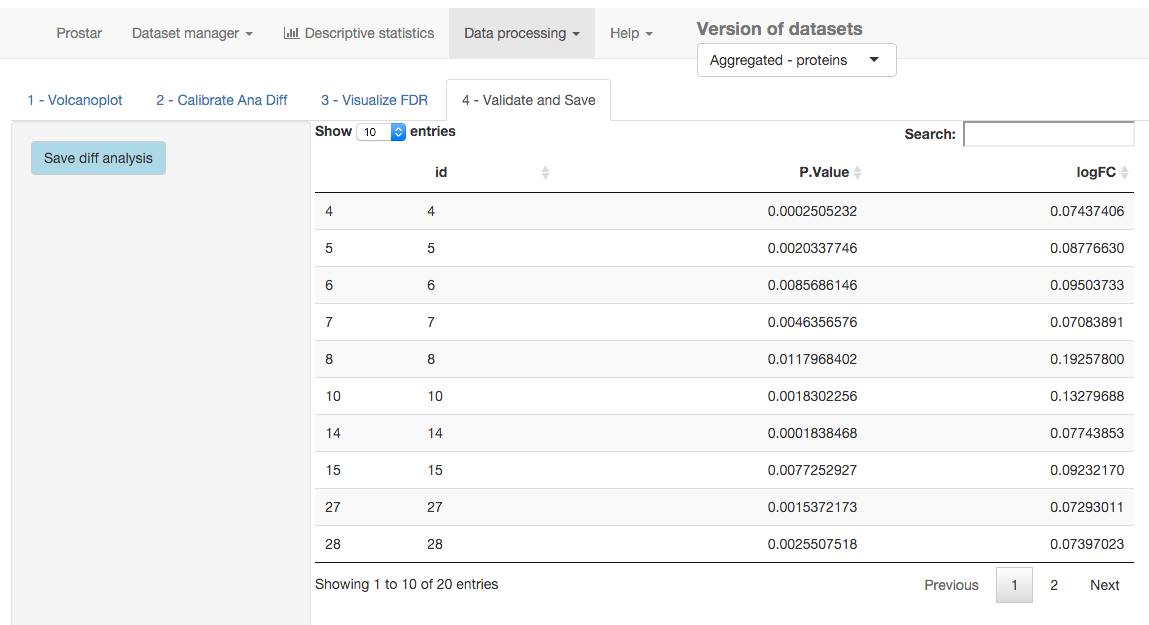
\includegraphics[width=\textwidth]{images/anaDiff4.png}}
\caption{Table of the results of statistical test in the differential 
analysis tool.}\label{fig:anadiff4}
\end{figure}

\hl{\bf Command line:} The \Biocpkg{DAPAR} functions for the Welch $t$-test 
and moderated $t$-test are \Rfunction{diffAnaWelch()} and 
\Rfunction{diffAnaLimma()}, respectively. These functions return a 
\Rcode{data.frame} which contains 2 columns: the p-values and the Fold Change 
of the test. These columns can be added to the current MSnSet object 
\Robject{imputed\_dataset} (as explained earlier) with the function 
\Rfunction{diffAnaSave()}:
\begin{Schunk}
\begin{Sinput}
> res <- diffAnaLimma(imputed_dataset, condition1, condition2)
> obj <- diffAnaSave(imputed_dataset, res, "limma", condition1, condition2)
\end{Sinput}
\end{Schunk}
Moreover, \Rfunction{diffAnaSave()} adds the aforementioned third column 
named "Significant" to the MSnSet object. Two optional arguments allows the 
user defining the thresholds on the $p$-values and on the Fold Change, so has 
to be more or less stringent on the number of proteins called "Significant".





%%%%%%%%%%%%%%%%%%%%%%%%%%%%%%%%%%%%%%%%%%%
%% Menu
%%%%%%%%%%%%%%%%%%%%%%%%%%%%%%%%%%%%%%%%%%%
\subsection{Help}
The Help screen offers various information:
\begin{itemize}
\item\textbf{{The MSnSet format}}. On this screen, there is a link to an 
article about the MSnSet format in order to explain its architecture to the 
user,
\item\textbf{{Refs}}. The references associated and/or related to the 
packages \Biocpkg{DAPAR} and \Biocpkg{ProStaR}.
\end{itemize}


%%%%%%%%%%%%%%%%%%%%%%%%%%%%%%%%%%%%%%%%%%%
%% Menu
%%%%%%%%%%%%%%%%%%%%%%%%%%%%%%%%%%%%%%%%%%%
\subsection{Versions of dataset}\label{sec:availabledatasets}
This major element of the Dataset manager is not in the corresponding menu, 
but on the contrary is detached on the right hand side of the navbar. The 
reason is,  it is convenient to have a constant view on it. It is a drop-down 
menu that lists the different versions of dataset of interest, i.e. the 
restauration points that were progressively saved along the quantitative 
analysis. 

Basically, each time the modifications of the current dataset are saved, the 
new dataset does not overwrite the previous one. On the contrary, the 
different versions are stored in memory. Thus, \Biocpkg{ProStaR} keeps a 
history of all processing performed on a dataset. Concretely, right after 
creating or uploading a dataset, only a single dataset is available: it is 
named "Original (peptide)" or "Original (protein)" depending on the data 
being related to peptides or proteins. This information is registered in the 
MSnSet file (the slot "typeOfData" of \Rfunction{experimentData(object)}). 
After the filtering step, if the user saves his/her results, another dataset 
becomes available, named "Filtered (peptide)" or "Filtered (protein)". 
Similarly, after the saving of the normalization, of the imputation of 
missing values, of the aggregation into proteins and of the differential 
analysis, a new dataset is created and stored. Each time a new dataset is 
created, it is by default the one on which the processing goes on. However, 
the previous one is accessible through the "Dataset versions" drop-down menu.

{At any time, the name of the current dataset and the type of data are 
displayed. If the user needs to return to a previous dataset (for example, 
the current dataset is "Imputed" and the user wants to return to "Filtered"), 
he/she chooses it in the select field. The dataset is then automatically 
loaded in memory and becomes the current one; the new dataset becomes the new 
current one. Naturally, all the plots that are displayed throughout the 
various panels of \Biocpkg{ProStaR} are dynamically updated without any 
action from the user.}


\textbf{Remarks:}
\begin{itemize}
%\item If the user chooses a dataset within those available, the dataset is 
%not directly reloaded as the working one. To do so, it is mandatory to click 
%on "Refresh dataset". %After this, the dataset which is highlighted in the 
%menu is the one which is worked on in the current session.
\item Let us note that if the user saves the current step (let us say the 
imputation step), then goes back to a previous step (say the normalization 
step) and start working on this older dataset (for instance, by performing 
another imputation) and then saves it, the new version of the processing 
overwrites the previous version (the older imputation is lost and only the 
newest one is stored in memory): in fact, only a single version of the 
dataset can be saved for a given processing step.
\item For a refined analysis regarding the influence of a processing step, 
it also possible to switch from an older to a newer dataset (that has been 
saved before) with the "Dataset versions" drop-down menu, and to observe the 
variations in the "Descriptive statistics" menu.
\end{itemize}

%The "Clear all" button deletes all the Available datasets. 


%%%%%%%%%%%%%%%%%%%%%%%%%%%%%%%%%%%%%%%%%%%
%% Section
%%%%%%%%%%%%%%%%%%%%%%%%%%%%%%%%%%%%%%%%%%%

\section{Bugs}\label{sec:sessionBugs}

Both packages \Biocpkg{DAPAR} and \Biocpkg{Prostar} are under active 
development. Despite our attention bugs may remain. To signal any, as well 
as typos, suggestions, etc. or even to ask a question, please contact us by 
email. Please join to the message as much information as possible, a 
reproducible example and the output of sessionInfo(). 

Here follow some error messages that the user may encounter and the tip to 
work around (please note that this section will be enriched with your 
feedbacks):


%%%%%%%%%%%%%%%%%%%%%%%%%%%%%%%%%%%%%%%%%%%
%% Section
%%%%%%%%%%%%%%%%%%%%%%%%%%%%%%%%%%%%%%%%%%%

\section{Session information}\label{sec:sessionInfo}
\begin{itemize}\raggedright
  \item R version 3.4.2 Patched (2017-10-08 r73502), \verb|x86_64-apple-darwin15.6.0|
  \item Locale: \verb|fr_FR.UTF-8/fr_FR.UTF-8/fr_FR.UTF-8/C/fr_FR.UTF-8/fr_FR.UTF-8|
  \item Running under: \verb|macOS Sierra 10.12.6|
  \item Matrix products: default
  \item BLAS: \verb|/Library/Frameworks/R.framework/Versions/3.4/Resources/lib/libRblas.0.dylib|
  \item LAPACK: \verb|/Library/Frameworks/R.framework/Versions/3.4/Resources/lib/libRlapack.dylib|
  \item Base packages: base, datasets, graphics, grDevices, methods,
    stats, utils
  \item Loaded via a namespace (and not attached): backports~1.1.1,
    BiocStyle~2.5.40, compiler~3.4.2, digest~0.6.12, evaluate~0.10.1,
    htmltools~0.3.6, knitr~1.17, magrittr~1.5, Rcpp~0.12.13,
    rmarkdown~1.6, rprojroot~1.2, stringi~1.1.5, stringr~1.2.0,
    tools~3.4.2, yaml~2.1.14
\end{itemize}
%\bibliography{\Biocpkg{ProStaR}}


\end{document}
